%%
%% DOCUMENT TYPE
%%

% general options:
% - inputenc        file encoding (should be "utf8" in most cases)
% - de/en           language of your work (influence pre-defined tokens)
% - declaration     adds the mandatory statutory declaration for theses
% - abstract        adds the abstract (from file "prelude_abstract.tex")
% - acknowledgment  adds an acknowledgment (from file "prelude_acknowledgment.tex")
%                   it is a nice gesture to personally thank people who
%                   supported you during your work.
% - symbollist      adds a list of symbols (from file "prelude_symbols.tex")
% - figurelist      adds and automatically creates a list of figures 
% - tablelist       adds and automatically creates a list of tables
% - index           generates an index based on the package "makeidx", please
%                   refer to its documentation for usage on index markup
% - bibbacklinks    adds backlinks from bibliography to the pages, where the
%                   corresponding entry is used (cited)
% - gray            make a gray-style version of the thesis report
%
% PhD thesis specific options
% - cv              adds your cv
% - publishsize     changes the page size from A4 to A5 for print publishing
%                   (please change the font size to 9pt, if you use this option)
% - approved        use this option, after your thesis has been formally approved
%                   (this will change the front page to meet formal/legal requirements)
% - ownpub          adds a second bibliography (from file "ownpub.bib") for your own
%                   publications related to the PhD thesis. According to the latest
%                   examination regulations, own work should be part of the regular
%                   bibliography (this option is hence obsolete)

\documentclass[de,acronymlist,declaration,bibbacklinks,inputenc=utf8]{tuhhthesis}
%\documentclass[de,acknowledgment,declaration,abstract,symbollist,inputenc=utf8]{tuhhthesis}


% for the acronyms
% - footnote        die Langform als Fußnote ausgeben
% - nohyperlinks    wenn hyperref geladen ist, wird die Verlinkung unterbunden
% - printonlyused   nur Abkürzungen auflisten, die tatsächlich verwendet werden.
%    Im printonlyused-Modus kann zusätzlich noch die Option withpage verwendet werden. Hierdurch wird im Abkürzungsverzeichnis zusätzlich die Seitenzahl, auf welcher die Abkürzung als erstes verwendet wurde, ausgegeben.
% - smaller         Text soll kleiner erscheinen, das Paket relsize wird vorausgesetzt
% - dua             es wird immer die Langform ausgegeben
% - nolist          es wird keine Liste mit allen Abkürzungen ausgegeben
\usepackage[printonlyused, withpage]{acronym}


%%
%% SETUP BLOCK
%%

% thesis type, must be one of the following
% - projectwork
% - bachelorthesis
% - masterthesis
% - diplomathesis
% - phdthesis
\setthesistype{bachelorthesis}

% your full name as printed on any official document (e.g., passport)
\author{Niklas Joachim Eberhard Krüger}

% the official title of your work (*must* match the filed title)
\title{Reverse Engineering eines Kaffeevollautomaten}

% the institution of the first examiner (refer to tuhhlangnames.def)
\institute{InstTelematics}

% date of submission as DD.MM.YYYY
\submitdate{22.02.2019}

% your matriculation number (for anything but PhD thesis)
\matrnumber{21491319}

% your course of studies
\course{Informatik-Ingenieurwesen}

% full name and affiliation of first and second examiner
\examinerFirst{Prof. Dr. Volker Turau}{Institut für Telematik\newline Technische Universität Hamburg}
\examinerSecond{Florian Meyer}{Institut für Telematik\newline Technische Universität Hamburg}

\supervisorFirst{Florian Meyer}{Institut für Telematik, Technische Universität Hamburg}
%\supervisorSecond{Volker Turau}{Institute of Telematics, Hamburg University of Technology}

% optional: print the TUB document number on title page
% this only applies, if the document is formally publish under
% a TUB document number
%\tubdoknumber{4711}


% Curriculum Vitae
% only needed for thesis type PhD
%\usepackage[]{currvita}
%\setlength{\cvlabelwidth}{50mm}
%\renewcommand*{\cvlistheadingfont}{\normalfont\sffamily\large\color{tuhh_blue}}
%\renewcommand*{\cvlabelfont}{\normalfont\rmfamily\normalsize\color{tuhh_darkgray}}



%%
%% CONTENT AREA
%%

% mathematical symbols
% absolute value, ceiling, floor
\newcommand{\abs}[1]{\left|{#1}\right|}
\newcommand{\floor}[1]{\left\lfloor{#1}\right\rfloor}
\newcommand{\ceil}[1]{\left\lceil{#1}\right\rceil}

% regular sets %
\newcommand{\setN}{{\mathbb N}}
\newcommand{\setZ}{{\mathbb Z}}
\newcommand{\setQ}{{\mathbb Q}}
\newcommand{\setR}{{\mathbb R}}
\newcommand{\setC}{{\mathbb C}}
\newcommand{\classNP}{{\cal {NP}}}
\newcommand{\classP}{{\cal {P}}}

% a node and a sink
\newcommand{\node}{v}
\newcommand{\sink}{\node_{0}}          % sink

% Node Related Sets
\newcommand{\Network}{G}
\newcommand{\setNodes}{{\mathcal V}}% set of nodes
\newcommand{\setLinks}{{\mathcal E}}% set of edges
\newcommand{\setNeighbors}[1]{{\mathcal N}_{#1}}% neighbors
\newcommand{\setTree}{{\mathcal T}}% tree
\newcommand{\setChildren}{{\mathcal C}}%
\newcommand{\setLeafs}{{\mathcal F}}%
\newcommand{\numNodes}{N}%
\newcommand{\numChildren}{C}%

% density
\newcommand{\nodeDensity}{\varrho}

%% EOF


\newcommand{\todo}{\fcolorbox{black}{yellow}{\textcolor{red}{!!!ToDo!!!}}}

% ~/texmf/tex/latex/tuhh/tuhhcolor.sty
\newcommand{\wort}[1]{\textcolor{tuhh_darkturquoise}{#1$_{16}$}} % EEPROM
\newcommand{\bitTrue}[1]{#1: \wert{$0 \rightarrow 1$}}
\newcommand{\bitFalse}[1]{#1: \wert{$1 \rightarrow 0$}}
\newcommand{\immer}[1]{\TDc\underline{#1}} % RAM Status auch im ausgeschalteten Zustand
\newcommand{\geteilt}[1]{(#1)} % RAM Status Bit mit mehreren Bedeutungen
\newcommand{\bytebit}[2]{Byte \wort{#1} an Bit \textcolor{tuhh_darkturquoise}{#2}} % \bytebit{}{}
\newcommand{\bytebits}[3]{Byte \wort{#1} an den Bits \textcolor{tuhh_darkturquoise}{#2} und \textcolor{tuhh_darkturquoise}{#3}} % \bytebits{}{}{}
\newcommand{\bytebitss}[3]{Byte \wort{#1} an den Bits \textcolor{tuhh_darkturquoise}{#2} bis \textcolor{tuhh_darkturquoise}{#3}} % \bytebitss{}{}{}
\newcommand{\wert}[1]{\textcolor{tuhh_darkred}{#1}}
\newcommand{\bezeichnung}[1]{\underline{#1}}

\renewcommand{\TRhc}[3]{\multicolumn{#1}{#2}{\cellcolor{tuhh_gray}{#3}}} % Row Header for colored rows

\begin{document}

%\phantomsection%prevents "Warning: No destination for bookmark of \addcontentsline"
%\addchap{\tuhh@printTag{ListOfSymbols}}\label{Test}
%\begin{center}
\footnotesize
\begin{supertabular}{p{.4\textwidth}p{0.54\textwidth}}
\abovebodyrule
	$\setN, \setZ, \setQ, \setR, \setC$
	& Regular sets of numbers
\\\TRc
	$\classNP, \classP$
	& Complexity classes
\\
	$\setNodes = \{ \node_0,\ldots,\node_{\numNodes-1} \}$%
	& Set of $\numNodes$ nodes $\node_i$ belonging to a network with sink $\sink$
\\\TRc
	$\nodeDensity$%
	& Node density, i.e., the average number of nodes within another node's communication range
\\
	$(\node_i,\node_j) \in \setLinks$%
	& Set of bidirectional communication links in the network
\\\TRc
	$\Network = \left( \setNodes, \setLinks \right)$%
	& Graph representation of a wireless sensor network
\\
	$\setNeighbors{i} = \{ \node_j \in\setNodes \mid i\!\!\ne\!\!j \wedge (\node_i,\node_j) \in \setLinks \}$%
	& The set of bidirectional communication partners of node~$\node_i$
\\\TRc
	$\setTree \subseteq \setLinks, \quad \abs{\setTree} = \numNodes\!-\!1$%
	& Routing tree rooted in the sink
\\
	$\setTree_i$%
	& Subtree rooted in (and including) node $\node_i$
\\\TRc
	$\setChildren_i, \quad \numChildren_i=\abs{\setChildren_i}$%
	& The set and number of children of node $\node_i$ in $\setTree$
\\
	$\setLeafs=\{\node_i\in\setNodes\mid\setChildren_i=\emptyset\}$%
	& Set of leafs in $\setTree$ and the number of leafs
\\\TRc
	$\setLeafs_{i}$%
	& Set of leafs in the subtree $\setTree_i$ of $\setTree$
\\\belowbodyrule
\end{supertabular}
\end{center}

%\cleardoublepage

%\renewcommand\contentsname{\tuhh@printTag{LotName}}
%\listoftables
%\addcontentsline{toc}{chapter}{\tuhh@printTag{LotName}}
%\cleardoublepage

% The Chapters
\chapter{Einführung}
\todo Einleitungssätze.

\section{Motivation}
Heutige Geräte versprechen viel Komfort und eine einfache Handhabung. Über das Internet werden die Geräte zunehmend vernetzt und smart.
Diese Arbeit befasst sich mit einer Kaffeemaschine und in erster Linie mit ihrem Speicher. Dieser merkt sich nicht nur Betriebszustände,
sondern auch Einstellungen, Zählstände und evtl. vieles mehr. Diese Informationen können nicht nur gelesen, sondern zum Teil auch verändert werden.
Moderne Funktionen stecken ohne eine entsprechende graphische Schnittstelle aber bereits in älteren Maschinen, unter der Voraussetzung über das entsprechende Wissen zu verfügen.

\todo Deutlich mehr ausholen: Was ist IoT? Warum braucht man das? Warum ist das relevant für diese Arbeit? Und dann zur Aufgabenstellung überleiten.

\section{Aufgabenstellung}
Anhand eines \textit{Jura Impressa S9 Kaffeevollautomaten} soll der Speicher untersucht werden.
Welches Wort / Byte / Bit speichert welche Information? Welche Bedeutung haben diese auf den Betrieb?
Hierfür sollen Skripte erstellt werden und der Speicher systematisch untersucht werden.

Wenn die Denkweise der Kaffeemaschine bekannt ist, sollen Werte im \ac{EEPROM} abgefragt, aber auch gezielt verändert werden, sowie Statusinformationen aus dem \ac{RAM} ausgelesen werden.
Die erhaltenen Rohinformationen werden nach den gewonnen Erkenntnissen aufbereitet und stehen so für weitere Projekte zur Verfügung.

Als kleine Demonstrationen entsteht am Ende ein Programm, welches Profile anlegen kann, sodass jeder Nutzer auf Knopfdruck einen Kaffee nach seinen Lieblings Präferenzen zubereitet bekommt.

\todo Aufbau der Arbeit beschreiben: In Kapitel 2 werden grundlegende Begriffe erklärt und ein Einblick in den Stand der Technik gegeben...
 % Einführung
\chapter{Grundlagen}\label{ch:Grundlagen}
Dieses Kapitel differenziert den Begriff des \textit{Reverse Engineering} und zeigt weitere Arbeiten zu Kaffeemaschinen sowie intelligenten Geräten auf.

% Sektion {Literatur: was gibt es schon}
\section{Begrifflichkeiten}\label{sec:Begrifflichkeiten}
Der Titel dieser Arbeit lautet \texttt{Reverse Engineering eines Kaffeevoll-\\automaten}, aber hinter der Terminologie des Begriffs \textit{Reverse Engineering} steckt ein weites Spektrum an Bedeutungen.
E. J. Chikofsky und J. H. Cross differenzieren in ihrem Paper~\cite{43044} die Begriffe \textit{Forward Engineering}, \textit{Reverse Engineering}, \textit{Redocumentation}, \textit{Design Recovery}, \textit{Restructuring}, und \textit{Reengineering}.

Zugrunde liegt ein Produkt, welches während seiner Entwicklung mehrere Lebenszyklen durchlaufen hat.
Kassem A. Saleh beschreibt in seinem Buch~\cite{Solr-599853700} ausführlicher Entwicklungsaktivitäten, wie die Anforderungsanalyse, das Design, die Implementation, die Tests, die Installation und den Einsatz.
Während der Implementation nennt er Vorgehensmodelle der Softwareentwicklung, wie das Wasserfallmodell, den Prototypenbau, das Spiralmodell, den objektorientierten Ansatz, das inkrementelle und iterative Modell, sowie das agile Modell.
Jede (Hardware- und) Softwareentwicklung durchläuft dabei, unabhängig vom Modell, die verschiedenen Entwicklungsaktivitäten.
Das Voranschreiten zur nächsten Stufe, bis zur Fertigstellung des Produkts, stellt das \textit{Forward Engineering} dar.

Der zweite Begriff, das \textit{Reverse Engineering}, führt in die Gegenrichtung.
Aus dem implementierten Produkt wird auf das Design, bzw. aus dem Design auf die Spezifikationen geschlossen.
Dabei werden zum einen die Komponenten und ihr Zusammenspiel identifiziert, zum anderen wird aber immer eine höhere Abstraktionsebene, eine vorherige Stufe, rekonstruiert.
Ein wichtiges Zitat, welches in Abschnitt~\ref{sec:DiskussionBegriffReverseEngineering}  aufgegriffen wird, lautet: "`Reverse engineering in and of itself does not involve changing the subject system or creating a new system based on the reverse-engineered subject system.
It is a process of examination, not a process of change or replication."'\cite{43044}

\textit{Redocumentation} arbeitet auf einer Ebene und bringt primär eine andere Darstellung.
Das Paper nennt "`dataflow"', "`data structure"' und "`control flow"' als Beispiele, die über Werkzeuge wie Diagramm Generatoren, Syntaxhervorhebung und Querverweis Generatoren erzeugt werden können.
Das Kernziel sei es die Zusammenhänge und Ablaufpfade hervorzuheben.

Breiter angelegt ist das \textit{Design Recovery}, das für die Designwiederherstellung externe Informationen, Schlussfolgerungen, und Unschärfelogik mit einbezieht, um sinnvolle Abstraktionen auf höherer Ebene zu identifizieren, welche nicht aus dem System selbst hätten gewonnen werden können.

\textit{Restructuring} umfasst das Nachbauen einer Darstellung innerhalb einer Ebene.
Funktionalität und Semantik bleiben erhalten, während die Darstellung umgestaltet wird.
Als Beispiel wird die Umstellung von unstrukturiertem Spaghetti Code zu strukturiertem "`goto"' freien Code genannt.
Der Begriff umfasst auch Datenmodelle, Entwurfsmuster und Anforderungsstrukturen.
Dabei genügt das Wissen über die Struktur, ohne die Bedeutung dahinter zu verstehen, beispielsweise können "`if"' und "`case"' Ausdrücke ineinander überführt werden, ohne zu verstehen wann welcher Fall eintritt.
Normalerweise werden daher ohne Anpassung der Spezifikation keine Veränderungen vorgenommen.
\textit{Restructuring} ist oft eine Form der präventiven Instandhaltung.

Zuletzt wird der Begriff \textit{Reengineering} oder auch "`Renovation and Reclamation"' als nachträgliche, neu erstellte Form beschrieben.
Dafür geht \textit{Reverse Engineering} zum abstrakten Verständnis dem \textit{Forward Engineering} oder \textit{Restructuring} voraus.
Beim \textit{Reengineering} sind Anpassung der Spezifikation und Veränderungen durchaus möglich.
Ähnlich zum \textit{Restructuring} verändert das \textit{Reengineering} die unterliegende Struktur, ohne die Funktionalität zu beeinträchtigen.
Jedoch passiert es selten, dass beim \textit{Reengineering} keine weiteren Funktionalitäten hinzugefügt werden.
Damit ist der Begriff \textit{Reengineering} allgemeiner gefasst als das \textit{Restructuring}.
Aber \textit{Reengineering} ist kein Überbegriff für \textit{Reverse Engineering} und \textit{Forward Engineering}, nur weil es beides beinhaltet.
Beide Disziplinen entwickeln sich unabhängig vom \textit{Reengineering} weiter.

Auch K. A. Ingle~\cite{Solr-153077417} grenzt das Reverse Engineering von anderen Konzepten ab.
Das \textit{Reengineering} wird, im Gegensatz zu dem \textit{Reverse Engineering}, beschrieben als Neustrukturierung des Programmcodes ohne funktionale Änderungen am System.
Diese Beschreibung passt zum dem Begriff des \textit{Restructuring} aus dem Paper von E. J. Chikofsky und J. H. Cross~\cite{43044}.

Beim \textit{Simultaneous Engineering} greifen während einer Produktentwicklung mehrere Arbeitsabläufe frühzeitig verzahnt ineinander, um einen Zeitgewinn gegenüber eines traditionellen Projektablaufs zu erzielen.
Die schnelle und einfache Reproduzierbarkeit sei beispielsweise nicht das direkte Ziel des \textit{Reverse Engineering}, sondern ein Ziel des \textit{Simultaneous Engineering}, schreibt K. A. Ingle.
Dennoch könne aber die Idee des \textit{Simultaneous Engineering} in das \textit{Reverse Engineering} aufgenommen werden.

Eine weitere Differenzierung findet zwischen dem \textit{Hardware-} und dem \textit{Software Reverse Engineering} statt.
\textit{Software Reverse Engineeging} verfolgt das Ziel aus dem Programm Code ein übergeordnetes Design oder Spezifikationsangaben zu extrahieren.
\textit{Hardware Reverse Engineeging} hingegen befasst sich mit dem Fertigungs- oder Produktionssystem.
Das Buch von 1994 sah aber schon ein Zusammenwachsen beider Bereiche durch den Einsatz und die Einbettung von immer mehr Software in Hardwaresystemen kommen.
Die Relevanz des Reverse Engineering würde hoffentlich weiter steigen, um keine vorhandenen Softwaresysteme neu bauen zu müssen.
K. A. Ingle schreibt: "`The aim of reverse engineering is to increase productivity through improved documentation."'\cite{Solr-153077417}

Diese Arbeit greift den Gedanken auf und versucht den Einfluss und die Bedeutung einzelner Speicherstellen für weitere Arbeiten zu dokumentieren.

\section{Stand der Technik}
% Sektion (related work)
Eine Bachelorarbeit der Universität Magdeburg zum Thema "`Reverse-engineering a De'Longhi Coffee Maker to precisely bill Coffee Consumption"'\cite{BachelorarbeitDeLonghi} behandelt eine De'Longhi Kaffeemaschine.
Das Ziel ist es, den Verbrauch exakt zu bestimmen und das System damit um ein Abrechnungssystem zu erweitern.
Dafür wird eine \ac{MCU} über das \ac{SPI} zwischen Master und Slave Einheiten geschaltet und Informationen werden aus dem prorietären De'Longhi Protokoll ausgelesen.
Das Ergebnis der Arbeit ist unter anderem ein Verständnis über das interne Bus Protokoll der Maschine.
% ?! \todo https://www.cl.cam.ac.uk/coffee/qsf/coffee.html ?!

Ein Buch von E. Eilam~\cite{Solr-480966761} stellt den Begriff des Reverse Engineering ähnlich wie zu Beginn in Abschnitt~\ref{sec:Begrifflichkeiten} dar, geht aber im Folgenden tiefer auf das Reverse Engineering von Low-Level Software ein.
Ein Hauptaugenmerk des Buches liegt auf auf der sicherheitsrelevanten Seite sowie den Vorgänge und Lücken im Low-Level Bereich.

Diese Arbeit hingegen nutzt als Ansatz eine gegebene serielle Schnittstelle des Jura Kaffeevollautomaten mit einem ebenfalls proprietären \ac{UART} Protokoll.
Dabei wird aber nicht die Hardware geöffnet und beispielsweise die Firmware disassembliert und analysiert.

Soucek, Russ und Tamarit haben sich in ihrem Paper \cite{soucek2000smart} mit dem Aufbau eines Feldbusses befasst, um mehrere Küchengeräte zu vernetzen und über ein Gateway in das Internet zu bringen.

Diese Arbeit erstellt auf der Basis der Ergebnisse in Kapitel~\ref{ch:Ergebnisse} eine Schnittstelle für einen Computer, der wiederum als Server mehrere Endgeräte anbinden kann.
 % Grundlagen
% meine Arbeit deutlich vom gegebenen abgrenzen: Hard-&Software vs. meine Implementierung
\chapter{Hardware und Software}
Dieses Kapitel führt die gegebenen und verwendeten Hard- und Software Komponenten in dieser Arbeit auf.

\section{Der Kaffeevollautomat}
Der "`Jura Impressa S9"', siehe Abbildung \ref{subfig:Kaffeevollautomat}, ist ein Kaffeevollautomat mit fünf Kaffeebezugstasten: Spezialkaffee, 1 große Tasse Kaffee, 2 große Tassen Kaffee, 1 kleine Tasse Kaffee und 2 kleine Tassen Kaffee.
Auf der rechten Seite befinden sich Bedienelemente für heißes (Tee-)Wasser und Wasserdampf zum Milch Aufschäumen.
Der Kaffeevollautomat wird für seinen Betrieb direkt mit der Netzspannung versorgt.

% \begin{figure}
%   \begin{center}
%     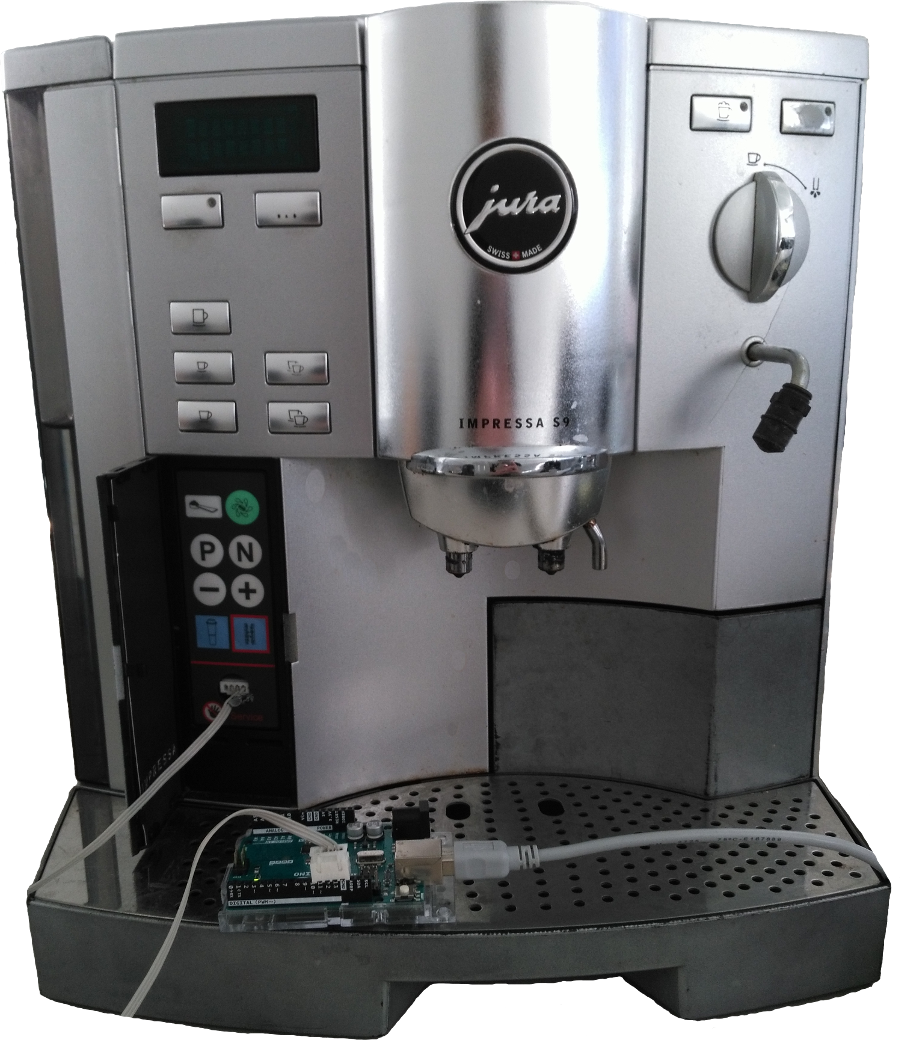
\includegraphics[scale=0.2]{images/Jura-Impressa-S9-small}
%     \caption{Jura Impressa S9 -- Kaffeevollautomat}
%     \label{fig:Kaffeevollautomat}
%   \end{center}
% \end{figure}

% \begin{figure}
%   \begin{subfigure}{.45\textwidth}
%     \centering
%     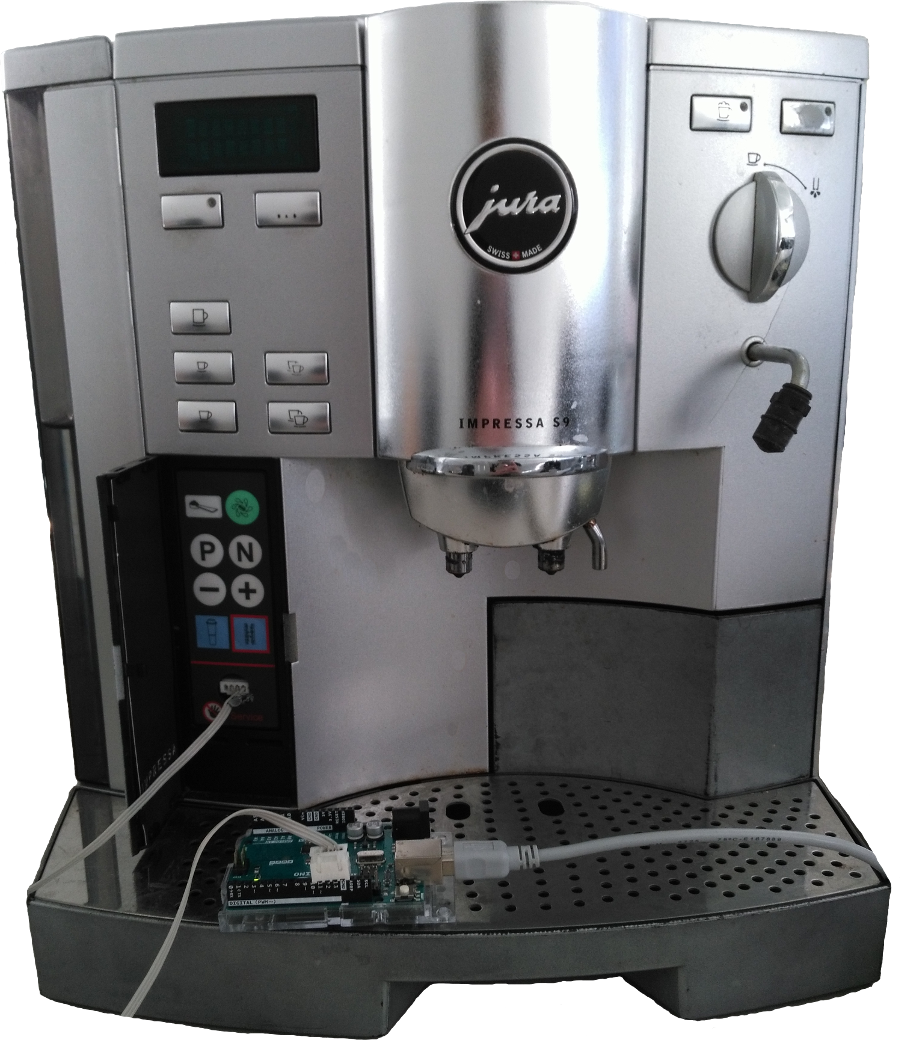
\includegraphics[scale=0.2]{images/Jura-Impressa-S9-small}
%     \caption{Jura Impressa S9 -- Kaffeevollautomat}
%     \label{fig:Kaffeevollautomat-xxxxxxxxxxxxxxxxxxxxxxxxxxxxxxxxxxxxxxxxxxxxxxxxxxxxxxxxxxxxxxxxxxxxxxxxxxxxxxxxxxxxxxxxxxx}
%   \end{subfigure}
%   \hfill
%   \begin{subfigure}{.45\textwidth}
%     \centering
%     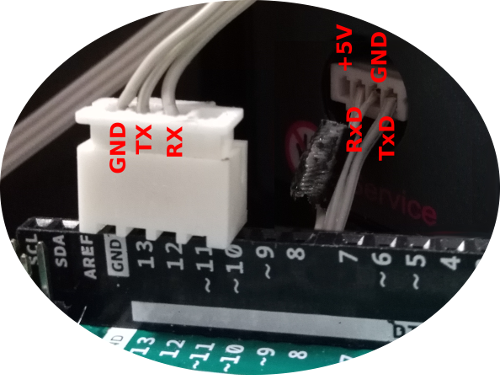
\includegraphics[scale=0.3]{images/Jura-Arduino-Pins-beschriftet-small}
%     \caption{Pinbelegung: Jura Impressa S9 -- Arduino Uno}
%     \label{fig:KaffeevollautomatPins-xxxxxxxxxxxxxxxxxxxxxxxxxxxxxxxxxxxxxxxxxxxxxxxxxxxxxxxxxxxxxxxxxxxxxxxxxxxxxxxxxxxxxx}
%   \end{subfigure}
% \end{figure}

\subfigbox{
  \subfigure[Der ganze Kaffeevollautomat]{\label{subfig:Kaffeevollautomat}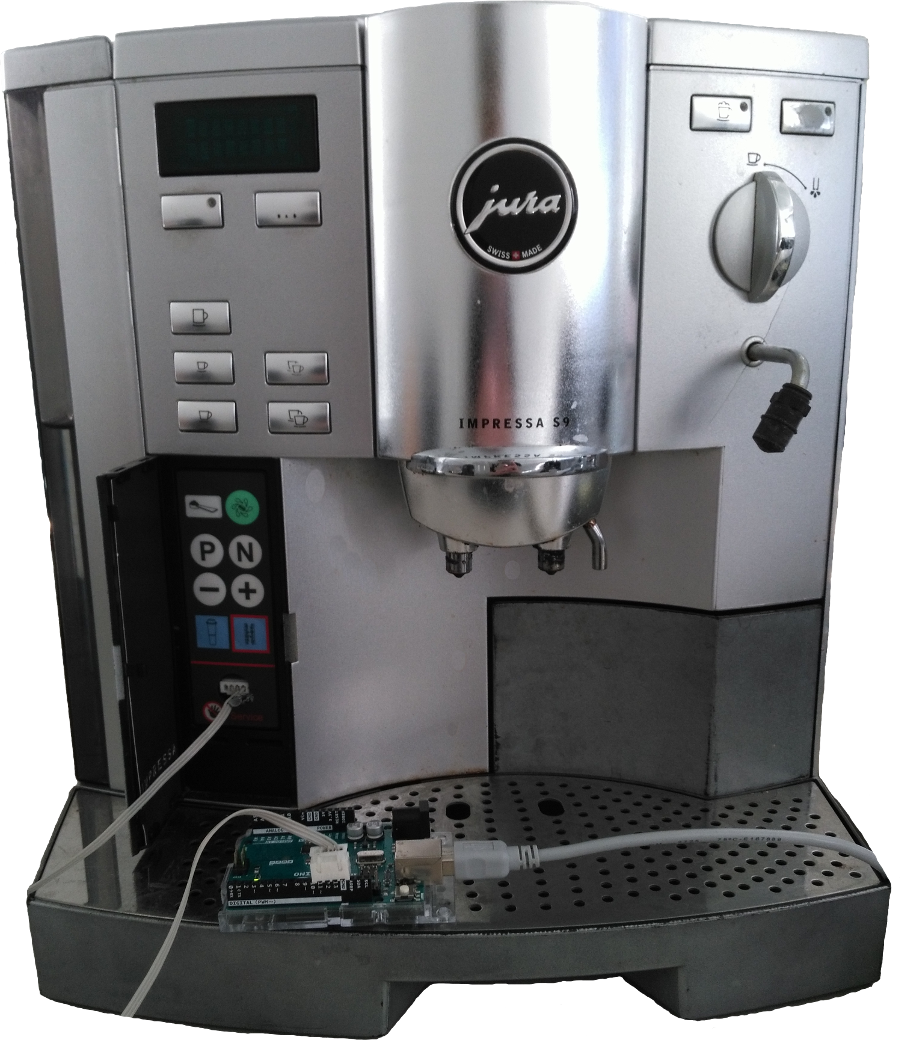
\includegraphics[scale=0.2]{images/Jura-Impressa-S9-small}}\hfill%
  \subfigure[Pinbelegung zum Arduino Uno]{\label{subfig:KaffeevollautomatPins}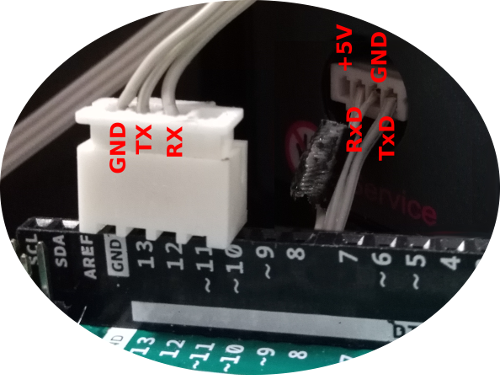
\includegraphics[scale=0.3]{images/Jura-Arduino-Pins-beschriftet-small}}%
}{Jura Impressa S9}{fig:Kaffeevollautomat}

\subsection{Aufbau und Verkabelung}
Hinter der linken Wartungsklappe an der Vorderseite des Kaffeevollautomaten befindet sich neben mehreren Menü-Tasten auch eine serielle Schnittstelle.
Über ein eigenes \ac{UART} Protokoll kann hierüber mit der Maschine kommuniziert werden.

Abbildung \ref{subfig:KaffeevollautomatPins} illustriert die Pinbelegung.
Die 5 Volt Leitung kann für ein autark laufendes Projekt genutzt werden.
In dieser Arbeit bezieht der Arduino seine Versorgungsspannung über den am USB Kabel befindlichen Computer.
Von \texttt{TX} nach \texttt{RxD} werden Befehle an den Kaffeevollautomaten verschickt.
Auf der Rückrichtung von \texttt{TxD} nach \texttt{RX} werden Antworten des Kaffeevollautomaten gelesen.
\texttt{GND} ist abschließend die gemeinsame Erdung und Bezugsleitung für die serielle Kommunikation.
Auf der Abbildung kreuzen sich die Leitungen \texttt{RxD} und \texttt{GND} am Stecker auf Seiten des Kaffeevollautomaten.
\texttt{GND} ist über eine schwarze Markierung gekennzeichnet.

Ein Arduino Uno übersetzt als "`Man in the middle"' die bekannten Kommandos in das Format der Kaffeemaschine.
Sie serielle Kommunikation läuft über die Pins Nummer 12 und 13.
Über eine weitere serielle Verbindung per USB lässt sich der Arduino ansteuern.

Aus Sicht des Computers ist der Arduino ein Gerätelaufwerk unter \texttt{/dev/ttyACM0} mit einer Baudrate von 9600.
Diese Zahl findet sich zu Beginn des Arduino Uno Skripts aus dem Projekt "`CoffeeMachine"'\cite{GitCoffeeMachine} wieder.

% \begin{figure}
%   \begin{center}
%     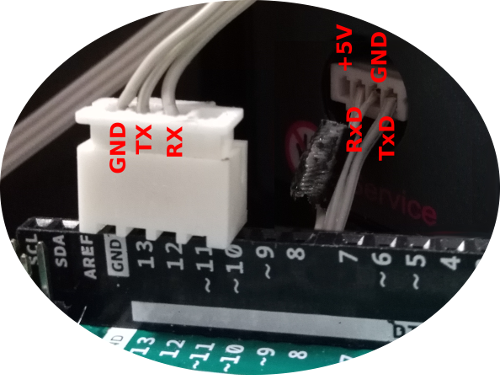
\includegraphics[scale=0.3]{images/Jura-Arduino-Pins-beschriftet-small}
%     \caption{Pinbelegung: Jura Impressa S9 -- Arduino Uno}
%     \label{fig:KaffeevollautomatPins}
%   \end{center}
% \end{figure}

\subsection{Kommandos}\label{subsec:Kommandos}
Die Tabelle~\ref{tbl:kommandos} zeigt die Befehlsgruppen, sowie ausgewählte Befehle, die der Kaffeevollautomat versteht.
Diese Befehle stammen aus dem Git Repository \cite{GitCoffeeMachine}, worauf diese Arbeit aufbaut.

Befehle beginnen entweder mit zwei Großbuchstaben gefolgt von einem Doppelpunkt und i.d.R. einer zweistelligen Hexadezimalzahl, oder sie beginnen mit einem Fragezeichen gefolgt von i.d.R. zwei ASCII Zeichen.
Positionsnummern, egal ob Speicherposition, \mbox{Betriebszustands-,} Bezugstasten- oder Steuerungskomponenten-Nummer, werden durch zweistellige Hexadezimalzahlen repräsentiert und reichen von $0_{16}=0_{10}$ bis FF$_{16}=255_{10}$.

Zwei Ausnahmen des ersten Typs sind z.B. \texttt{TY:} zum Abfragen des Maschinen Typs und \texttt{WE:00,01FF} zum Schreiben des Wertes $01$FF$_{16} = 511_{10}$ an die Position $00$.
Eine Ausnahme des zweiten Typs ist z.B. \texttt{?D1DISPLAY}\textvisiblespace\ und \texttt{?D2}\textvisiblespace\textvisiblespace\texttt{TEST}\textvisiblespace\textvisiblespace.
Der volle Umfang möglicher Displayzeichen, sowie deren Benutzung wird in Abschnitt \ref{sec:Display} ausgeführt.

Einige Befehle, die aus weiteren Projekten mit Maschinen der S-Reihe bekannt sind, sind in dieser "`Jura Impressa S9"' leider nicht implementiert.
Dazu zählen \texttt{IC:} zum Auslesen aller Eingaben, \texttt{FA:0A} eine unbelegte Bezugstaste, \texttt{CM:} für weitere Status Informationen, \texttt{CS:} für Sensor Informationen und \texttt{PM:} ein Befehl um Musik abzuspielen.
Weitere Befehlsgruppen werden in der \texttt{README.rst} eines Github Repositories aufgeführt\footnote{\url{https://github.com/PromyLOPh/juramote}}.

\begin{tuhhtable}
  \footnotesize\centering
  \begin{tabular}[tp]{L{.22\textwidth}L{.48\textwidth}L{.18\textwidth}}
%
  \THc{1}{c}{Kommando} & \THc{1}{c}{Beschreibung} & \THc{1}{c}{Rückgabewert} \\
%
  \TRx{3}{l}{Betriebszustand (AN:<id>)}\\
  \abovebodyrule
  AN:01    & Einschalten        & ok:    \\\TRc
  AN:02    & Ausschalten        & ok:    \\
  AN:03    & Display Test       & ok:    \\\TRc
  AN:<id>  & u.v.m.             & ok:    \\
  \belowbodyrule
%
  \TRx{3}{l}{Bezugstaste (FA:<id>)}\\
  \abovebodyrule
  FA:02    & Gerät spülen       & ok:    \\\TRc
  FA:0C    & Spezialkaffee      & ok:    \\
  FA:<id>  & u.v.m.             & ok:    \\\TRc
  \belowbodyrule
%
  \TRx{3}{l}{Steuerungskomponenten (FN:<id>)}\\
  \abovebodyrule
  FN:<id>  & Pumpen, Heizung, u.v.m & ok:    \\\TRc
  \belowbodyrule
%
  \TRx{3}{l}{Eingabestatus*}\\
  \abovebodyrule
  IC:      & Eingaben auslesen* &        \\\TRc
  \belowbodyrule
%
  \TRx{3}{l}{Spiele Musik (easter egg)*}\\
  \abovebodyrule
  PM:      & Play music*        &        \\\TRc
  \belowbodyrule
%
  \TRx{3}{l}{Speicherzugriff}\\
  \abovebodyrule
  RE:<address> & Liest 2 Byte EEPROM Speicher   & re:[0000-FFFF] \\\TRc
  WE:<address>,<value> & Schreibt 2 Byte in EEPROM & ok:         \\
  RT:<address> & Liest eine Zeile EEPROM        & rt:[0-F 64x]   \\\TRc
  RR:<address> & Liest eine Zeile RAM           & rr:[0-F 32x]   \\
  \belowbodyrule
%
  \TRx{3}{l}{Sperrung}\\
  \abovebodyrule
  ?M3      & Aktiviert den Inkassomodus         & ?ok            \\\TRc
  ?M1      & Deaktiviert den Inkassomodus       & ?ok            \\
  \belowbodyrule
%
  \TRx{3}{l}{Display}\\
  \abovebodyrule
  ?D0      & Standard Displaytext zurück setzen & ?ok            \\\TRc
  ?D1[A-Z 8-11x] & Displaytext Zeile 1          & ?ok            \\
  ?D2[A-Z 8-11x] & Displaytext Zeile 2          & ?ok            \\\TRc
  \belowbodyrule
%
  \TRx{3}{l}{Aktion an der Kaffeemaschine}\\
  \abovebodyrule
           & 1 kleiner Kaffee (Produkt 1)       & ?PAE         \\\TRc
           & 2 kleine Kaffees (Produkt 2)       & ?PAF         \\
           & 1 großer Kaffee  (Produkt 3)       & ?PAA         \\\TRc
           & 2 große Kaffees  (Produkt 4)       & ?PAB         \\
           & Spezialkaffe     (Produkt 7)       & ?PAG         \\\TRc
           & Dampf            (Produkt 6)       & ?PAI         \\
           & 1 Dampfportion   (Produkt 5)       & ?PAJ         \\\TRc
           & 1 Tasse Tee      (Produkt 8)       & ?PAK         \\
  \belowbodyrule
%
  \TRx{3}{l}{* leider nicht alles in der Jura Impressa S9 implementiert, siehe weitere Geräte der S-Reihe}\\
%
  \end{tabular}
  \caption{Befehlsübersicht der Jura Kaffeevollautomaten (S-Reihe)}
  \label{tbl:kommandos}
\end{tuhhtable}

\subsection{Serielle Kommunikation}
Das Arduino Skript aus dem Projekt "`CoffeeMachine"'\cite{GitCoffeeMachine} wird als Grundlage der Kommunikation in dieser Arbeit weiter verwendet.
Es kodiert die \ac{UART} Kommandos von und zu dem Kaffeevollautomaten.

Die Befehle aus der Kommando Tabelle~\ref{tbl:kommandos} werden zeichenweise ASCII-Zeichen für Zeichen übertragen.
Dafür wird ein an den Kaffeevollautomaten adressiertes Byte (ein ASCII-Zeichen), bestehend aus acht Bits, in je vier Bytes aufgeteilt.
Die dritte und sechste Stelle der neuen Bytes repräsentieren je zwei Bits des ursprünglichen Bytes.
Bei der Übertragung an den Kaffeevollautomaten werden die restlichen Bits mit Nullen aufgefüllt.
Abbildung \ref{fig:uart} veranschaulicht dies an dem ersten Byte des Einschaltbefehls, die entsprechende ASCII-Kodierung ist in Abbildung \ref{tbl:Displaysymbole} der zweiten und dritten Spalte zu entnehmen.
Die Kodierung der, von dem Kaffeevollautomaten kommenden, Bytes erfolgt analog.
Laut "`Protocoljura"'\footnote{\url{http://protocoljura.wiki-site.com/index.php/Protocol_to_coffeemaker}} bestehen die irrelevanten Bits der ankommenden Bytes aus einer Null und weiteren fünf Einsen pro Byte.

Vier Bytes kodieren auf diese Weise ein ASCII Zeichen und werden fortan als Gruppe bezeichnet.
Zwischen jeder Gruppe gibt es eine Verzögerung von 8ms.
Diese Verzögerung begrenzt hauptsächlich die Übertragungsgeschwindigkeit, was in Abschnitt \ref{subsec:zugangSeriellDirekt} diskutiert wird.

Die jetzt vorhandene Umgebung kann bereits über den seriellen Monitor der Arduino IDE genutzt werden.

\begin{figure}
  \begin{center}
    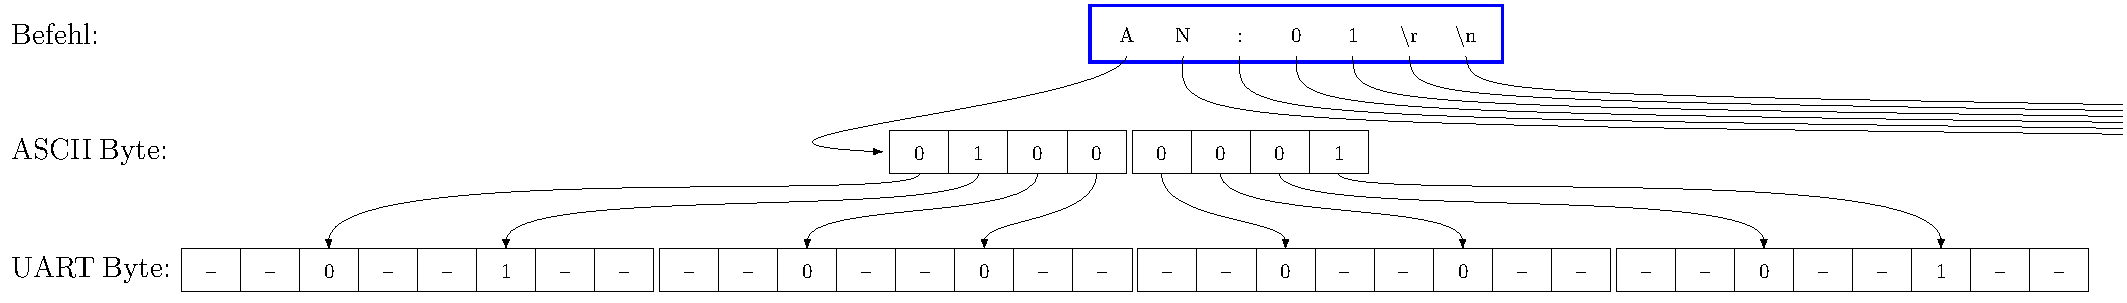
\includegraphics[scale=0.6]{images/UART-Bytes}
    \caption{Umrechnung }
    \label{fig:uart}
  \end{center}
\end{figure}



\section{Libraries und Frameworks}
Diese Arbeit nutzt "`libraries"' und "`frameworks"'.
"`libraries"' sind thematisch gebündelte Funktionen und Routinen. Sie bieten eine \ac{API}, die das eigene Programm ansprechen kann.

"`frameworks"' sind noch mehr und bieten ganze Programmiergerüste und Routinen. Sie rufen wenn nötig selbst vorgesehene Funktionen auf und folgen damit dem Paradigma des "`Inversion of Control"'.

In der aktuellen Version bieten beide nicht nur leicht zugängliche Aufrufe, sondern sind auch sicher und robust in ihrem Gebiet.

\subsection{Serielle Kommunikation}
Bei dem Versuch die Grätedatei direkt anzusprechen kam es zu Problemen, die in Abschnitt~\ref{subsec:kommunikationGeraetedateiLibserialLibrary} erörtert werden. Für die zuverlässige serielle Kommunikation kommt daher eine geeignete Library zum Einsatz.

\subsubsection{libserial}
Das selbst entwickelte C++ Programm nutzt "`liberial"'\footnote{\url{https://github.com/crayzeewulf/libserial}} um sicher und zuverlässig über das Gerätelaufwerk mit dem Arduino (und letztlich dem Kaffeevollautomaten) zu kommunizieren.
Diese Bibliothek bietet eine objektorientierte Schnittstelle für alle \ac{POSIX} Systeme und ist unter Linux über die Paketverwaltung installierbar.

\subsection{Speicher- und Austauschformat}
Sowohl bei der Untersuchung des Speichers, als auch am Ende für das aufbereitete Ergebnis, werden Informationen gesammelt, verglichen und öffentlich zugänglich gemacht.
Als beliebtes und flexibles Speicherformat wird \ac{JSON} verwendet.
Es bietet viele Datenformate und ist unbegrenzt verschachtelbar.
In dieser Arbeit werden hauptsächlich Zeichenketten, Zahlen, Unter-Objekte und -Arrays verwendet.

Darüber hinaus kann es leicht vom C++ Programm, der Webseite, oder auch für viele weitere Projekte genutzt werden.

\subsubsection{libjsoncpp}
Die "`libjsoncpp"'\footnote{\url{https://en.wikibooks.org/wiki/JsonCpp}} bietet dem C++ Programm eine Lese- und Syntaxanalyse-Funktion zum Aufnehmen eines \ac{JSON} Ausdrucks, sowie eine Möglichkeit ein \ac{JSON} Objekt kompakt zusammengefasst oder leserfreundlich aufgefächert in einen Ausgabestrom zu schreiben.
Als Ausgabestrom sind reine \ac{JSON} Dateien nach einer Speicherauszugs Aufnahme oder die Standardausgabe im Gebrauch als API vorstellbar.


\subsection{Webseite}
Eine kleine Webseite soll am Ende die ausgelesenen Werte visuell anschaulich präsentieren.
Die JavaScript-Bibliothek jQuery und das Framework Bootstrap helfen dabei dies zügig und ansprechend umzusetzen.

\subsubsection{Bootstrap}
Bootstrap\footnote{\url{https://getbootstrap.com/}} ist ein von den Twitter Entwicklern begonnenes Projekt um ursprünglich intern die Verwaltungswerkzeuge zu vereinheitlichen.
Daraus ist aber ein ganzes System an Design Elementen geworden, welches heute sehr populär ist.
\ac{HTML}, \ac{CSS} und \ac{JS} werden zusammen eingesetzt und bieten Entwicklern eine Gitteranordnung für eine Mobile- und die Desktop-Ansicht, Inhaltselemente wie Tabellen und Abbildungen oder auch einzelne Komponenten wie Steckkarten, Prozentanzeigen und Knöpfe.

\subsubsection{jQuery}
jQuery\footnote{\url{https://jquery.com/}} ist eine freie \acl{JS}-Bibliothek, die in der "`slim"'-Variante bereits über Bootstrap eingebunden ist.
Um später wirklich mit dem Kaffeevollautomaten interagieren zu können, wird unter anderem \acs{AJAX} aus dem vollständigen jQuery Paket benötigt (auch wenn daraus später ein synchrones JavaScript mit \acs{JSON} wird).

Über das \acs{CDN} eingebundene Packet stehen ab jetzt einfache \aclp{API} zum modifizieren der \acs{HTML} Elemente, ein erweitertes Event-System, sowie \acs{AJAX}-Funktionalitäten bereit.

\subsubsection{Intro.js}
Zu guter Letzt folgt mit Into.js\footnote{\url{https://introjs.com/}} noch eine Schritt-für-Schritt-Anleitung, die dem Seitenbenutzer eine kurze Einführung in den Aufbau und die Bedienung der Webseite geben soll.
 % Hardware und Software
\chapter{Methodik und Implementierung}
Dieses Kapitel führt das Vorgehen und die Implementierung eines C++ Programms aus, die es ermöglichen Aussagen über den Speicher des Kaffeevollautomaten zu treffen.
Immer wiederkehrende Arbeitsabläufe werden von diesem Programm übernommen und auf den unteren Ebenen automatisiert.

\section{Vorgehen}
\todo Ähnlich zum Blackbox Testing in \cite{Solr-599853700} wird mit Ein- und Ausgabe des Kaffeevollautomaten gearbeitet, ohne sein Programm zu kennen (Blackbox Modell)\todo

Die Speicher des Kaffeevollautomaten, der \ac{EEPROM} und der \ac{RAM}, können Zeilenweise ausgelesen werden.
Der nötige Zugriff zum Auslesen kann auf zwei Arten erfolgen: direkt am Speicherstein auf der Hauptplatine oder seriell über die vorhandene \ac{UART} Schnittstelle, siehe Abschnitt~\ref{subsec:zugangSeriellDirekt}.
Im Folgenden erfolgt die Kommunikation über die \ac{UART} Schnittstelle und mithilfe der \textit{libserial}-Library.

Unabhängig voneinander wurden beide Speicher untersucht.
Ein eigens entwickeltes C++ Programm setzt die sechzehn Zeilen einer Speicherabfrage zu einem gesamten Speicherauszug zusammen.
Intern werden dabei je zwei Hexadezimalzahlen in eine ganzzahlige Dezimalzahl umgerechnet und in einem Vektor abgelegt.
Dadurch sind Position und Wert bekannt.

\begin{figure}
  \begin{center}
    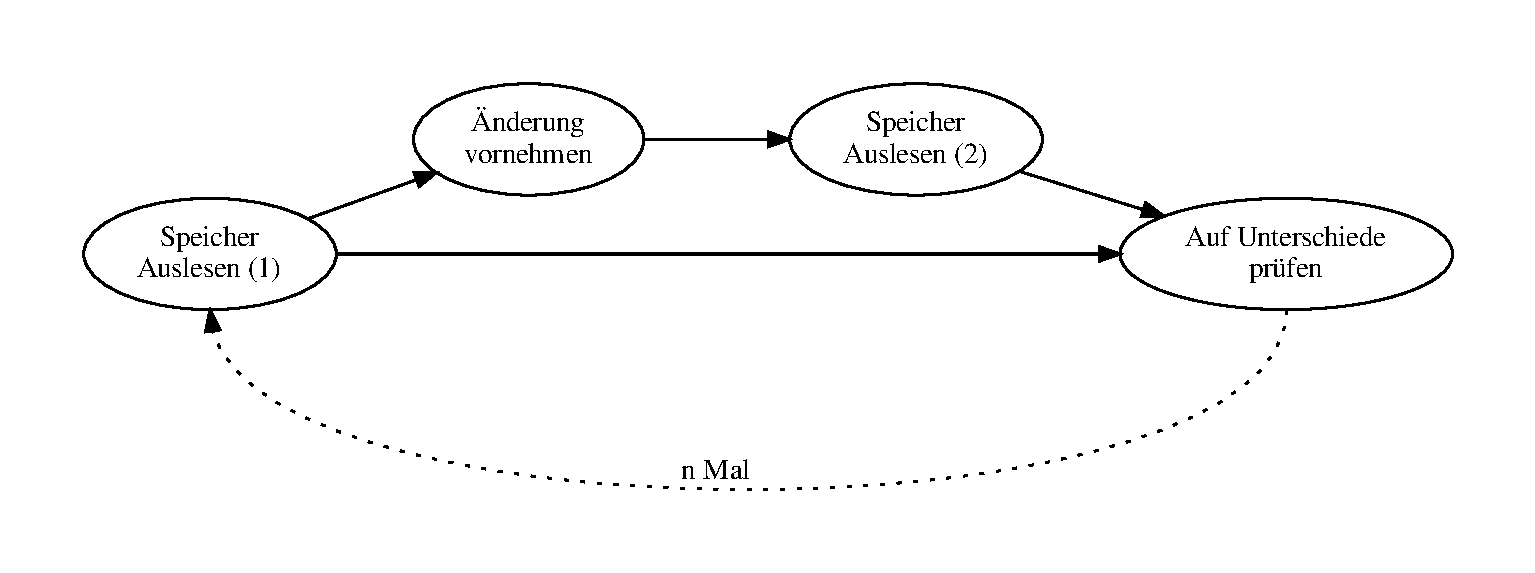
\includegraphics[scale=0.54]{images/chapter_4/workflow}
    \caption{Arbeitsablauf}
    \label{fig:workflow}
  \end{center}
\end{figure}

Abbildung~\ref{fig:workflow} visualisiert den Arbeitsablauf der zur Bestimmung der Speicherstellen in dieser Arbeit angewandt wurde.
Nach dem ersten Schritt ganz links wird nun von Hand eine möglichst elementare Veränderung an dem Kaffeevollautomaten vorgenommen, um gezielten Aktionen die Werteänderungen bestimmter Speicherzellen zuordnen zu können.
Die angewandten Veränderungen werden in Abschnitt~\ref{subsec:AenderungenAnDerMaschine} beschrieben.

Nach einer erneuten Aufnahme eines Speicherauszugs können diese beiden nun verglichen werden.
Das Programm iteriert durch den Vektor und vergleicht die Speicherwerte an der gleichen Position.
Bei Ungleichheit existiert ein Unterschied der festgehalten wird.
Dieser Ablauf wurde auf alle Einstellmöglichkeiten und Funktionen des Kaffeevollautomaten angewandt.

Bei dem \ac{RAM}, im Gegensatz zum \ac{EEPROM}, fiel jedoch auf, dass sich mehrere Speicherwerte auch ohne eine vorgenommene Veränderung änderten.
Deshalb wurden viele Speicherauszüge im Ruhezustand aufgenommen und die sich regelmäßig ändernden Bytes ausgeschlossen.
Zu Beginn der Ergebnisse über den \ac{RAM} in Abschnitt~\ref{sec:ErgebnisseRAM} sind diese aufgeführt.
Dennoch gab es gelegentliche Unregelmäßigkeiten, sodass das Vorgehen für den \ac{RAM} um eine geschlossene Rückrichtung ergänzt wurde.
In der Regel wurden pro \ac{RAM} Funktion $n=3$ Durchläufe vorgenommen und die gemeinsame Schnittmenge der Veränderungen bestimmt.

Ganz am Ende gab es noch ein zweites Vorgehen, bei dem gezielt der \ac{EEPROM} an bekannten Speicherstellen beschrieben wurde.
Hintergrund war die unbekannte Position bzw. später die Zusammensetzung des Bezüge-Zählers im Einstellungsmenü des Kaffeevollautomaten.
Abschnitt~\ref{subsec:Vorgehen2} führt dies im Folgenden aus.

\subsection{Veränderungen zur Bestimmung der Speicherstellen}\label{subsec:AenderungenAnDerMaschine}
\subfigbox{
  \subfigure[Fassung im Kaffeevollautomaten]{\label{subfig:fassung}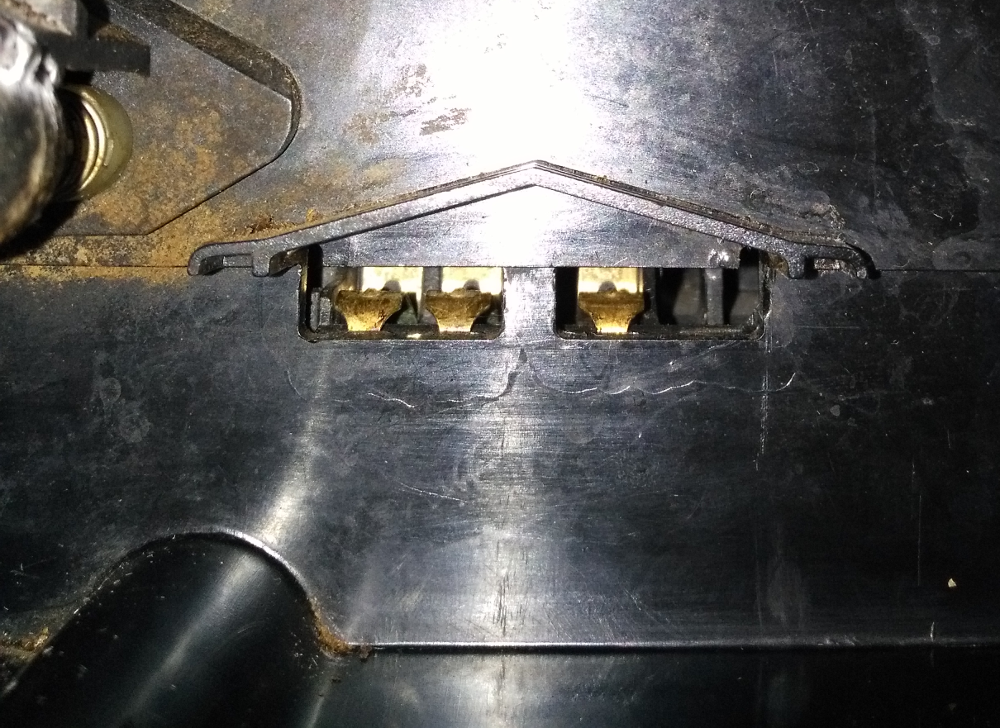
\includegraphics[scale=0.2]{images/chapter_4/Schale-Fassung}}\\%
  \subfigure[Oberseite des Schalen Ersatzes]{\label{subfig:oberseite}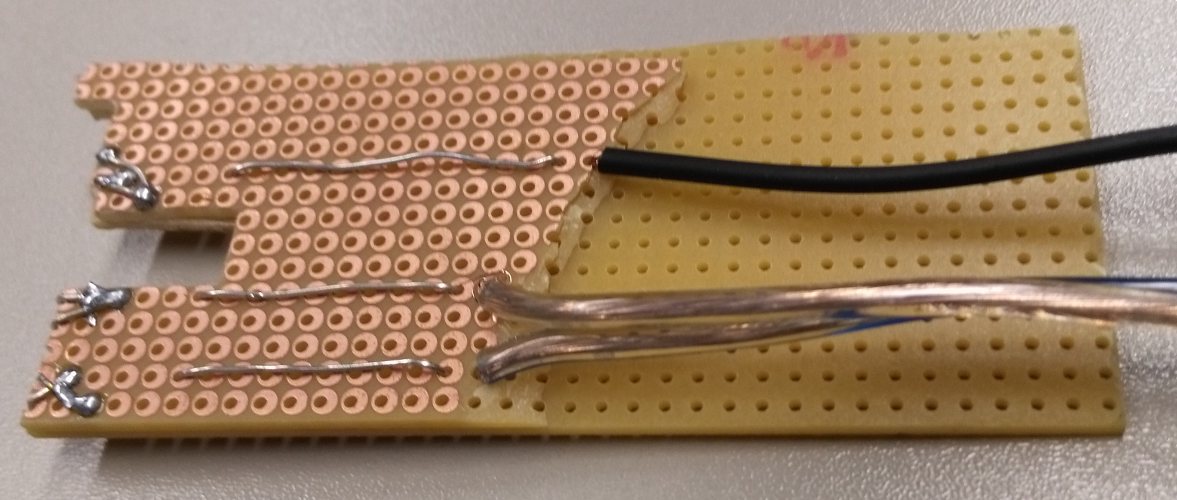
\includegraphics[scale=0.29]{images/chapter_4/Schale-Oberseite}}\\%
  \subfigure[Unterseite des Schalen Ersatzes]{\label{subfig:unterseite}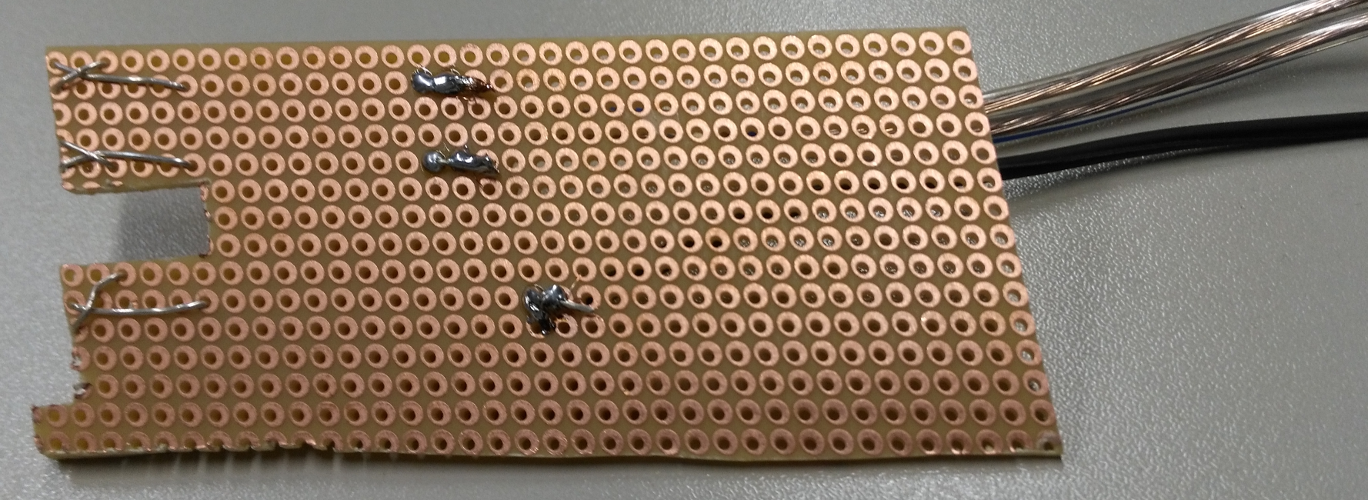
\includegraphics[scale=0.25]{images/chapter_4/Schale-Unterseite}}%
}{Ersatz der Schale des Kaffeevollautomaten}{fig:ersatzschale}

Für den \ac{EEPROM} war es hilfreich einmal das Handbuch der Maschine systematisch durch zugehen und zum Beispiel immer eine Menüoption zu variieren.
Bei einer Skala (wie z.B. beim Kaffeepulver) hat es ausgereicht den niedrigsten, den höchsten und den Standard-Wert im Speicher zu bestimmen;
deckte sich die einstellbare Anzahl an Abstufungen mit der Werte Differenz im Speicher, ließ sich auf die verbleibenden Werte schließen.
Auch im normalen Gebrauch fiel somit u.a. ein Einschaltzähler im \ac{EEPROM} auf.

Für den \ac{RAM} ging es mit den gezielt auslösbaren Statusmeldungen los.
Das Anheben des Wassertanks oder das Abziehen der unteren Schale löste eine Warnmeldung auf dem Display aus und wurde auch im \ac{RAM} vermerkt.
Ein zu hoher Wasserstand in der Schale konnte ohne Wasser mit einer eigenen Platine vorgegaukelt werden.
Abbildung~\ref{subfig:fassung} zeigt die Fassung an der Rückwand innerhalb des Kaffeevollautomaten für die Schale.
Abbildung~\ref{subfig:oberseite} und \ref{subfig:unterseite} visualisieren die Platine, an der leicht von außen mittels Krokodilklemmen die Kontakte im Inneren kurzgeschlossen werden konnten.
Am schwierigsten sind komplexe Abläufe, wie die Zubereitung eines Kaffees.
Hier konnte nur mehrfach zu gezielt gleichen oder ungleichen Zeitabständen der zweite Speicherauszug angestoßen werden.
Hier sei schon einmal der Verweis auf Abschnitt~\ref{sec:AussagekraftDerErgebnisse} zur Aussagekraft dieser Ergebnisse genannt worden.

Abschließend war auch für das Display ein kleines Programm nötig um die volle Funktionsvielfalt festzustellen.
Abschnitt~\ref{subsec:tools} führt dies später aus.

\subsection{EEPROM gezielt beschreiben}\label{subsec:Vorgehen2}
Ziel war es die unbekannte Position bzw. später die Zusammensetzung des Bezüge-Zählers im Einstellungsmenü des Kaffeevollautomaten zu entziffern.
Dafür wurde die angezeigt Zahl in eine Hexadezimalzahl umgerechnet und im Speicherauszug des \ac{EEPROM} des Kaffeevollautomaten gesucht.
Da die Zahl eine Stromunterbrechung überstand und eine Änderung des einzigen übereinstimmenden Wertependants in Wort \wort{15} keine Änderung der Ausgabe hervorrief, begann die Suche an weiteren bekannten Speicherstellen im \ac{EEPROM}.

Der Bezüge-Zähler setzt sich aus mehreren Zählern zusammen.
Der Trester Füllstand in der Schale wird nicht gemessen, sondern im Betrieb gezählt um den Füllstand zu erfassen.
Auch die Reinigungsankündigung beruht auf Zählständen über Kaffee Bezüge und Spülungen.
Die Wasser Durchflussmenge des Filters wird ebenfalls erfasst und ab einem festen Wert eine Warnmeldung zum Wechseln ausgegeben.

Das gezielte eingreifen in die Zählstände ließ es zu diese Grenzwerte zu bestimmen.
Die Ergebnisse befinden sich in Abschnitt~\ref{subsec:ErgebnisKaffeezubereitung}.

\section{Das C++ Programm "`./JuraCoffeeMemory"'}
Für diese Arbeit wurde ein C++ Programm entwickelt, das die Kommunikation und die Aufschlüsselung der Antworten übernommen hat.

\subsection{Makefile}
In dem Projekt Ordner befinden sich auf der Hauptebene mehrere \texttt{CPP}- und \texttt{HPP}-, eine \texttt{H}- sowie eine \texttt{Makefile}-Datei.
Sind die in der \texttt{Readme.md} genannten Abhängigkeiten und Voraussetzungen erfüllt, kann das Projekt mit dem Befehl \texttt{make}, ohne Zusatzangaben gebaut werden.
Am Ende sollte dann auf der Hauptebene eine ausführbare Datei namens \texttt{./JuraCoffeeMemory} herauskommen.
Es werden neben Objekt-Dateien auch noch einige weitere Tools im Unterordner \texttt{./tools/} gebaut, auf die später in Abschnitt~\ref{subsec:tools} eingegangen wird.

Der Befehl \texttt{make clean} entfernt die Objekt-Dateien, mittels \texttt{make dist-clean} werden ebenfalls die ausführbaren Programme entfernt und der Projekt Ordner in seinen Ursprungszustand zurück versetzt.

\subsection{Interaktives Menü}
Startet man in einem Terminal das Hauptprogramm \texttt{./JuraCoffeeMemory} wird das Hauptmenü angezeigt. Abbildung~\ref{subfig:terminal1-MainMenu} visualisiert diesen Zustand.
Das Listing~\ref{lst:menu-tree} zeigt einmal schematisch all Menüoptionen.

\subfigbox{
  \subfigure[Hauptmenü]{\label{subfig:terminal1-MainMenu}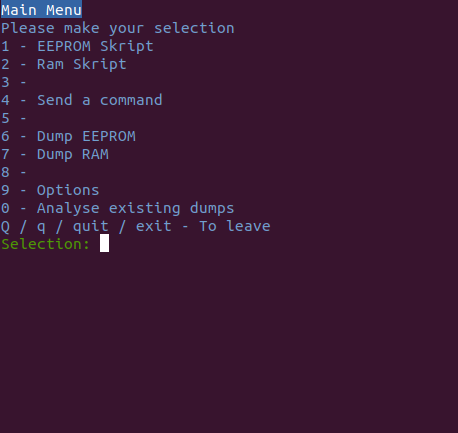
\includegraphics[scale=0.4]{images/chapter_4/JuraCoffeeMemory-1-MainMenu}}\hfill%
  \subfigure[Optionen $\leadsto$ Log Pfad ändern]{\label{subfig:terminal7-Options-RamLogFilePath}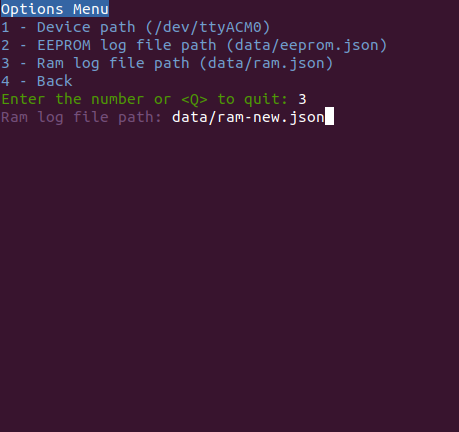
\includegraphics[scale=0.4]{images/chapter_4/JuraCoffeeMemory-7-Options-RamLogFilePath}}\\%
  \subfigure[RAM Speicherauszug]{\label{subfig:terminal5-RAM-dump}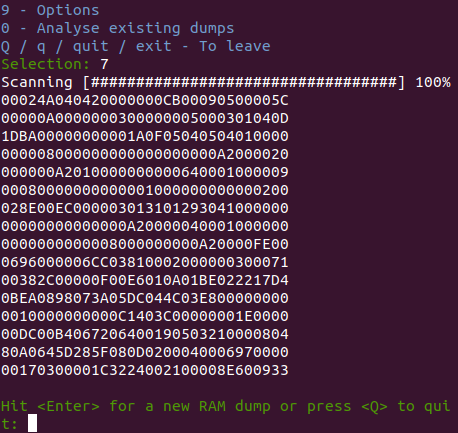
\includegraphics[scale=0.4]{images/chapter_4/JuraCoffeeMemory-5-RAM-dump}}\hfill%
  \subfigure[EEPROM Skript]{\label{subfig:terminal3-EEPROM-NothingChanged}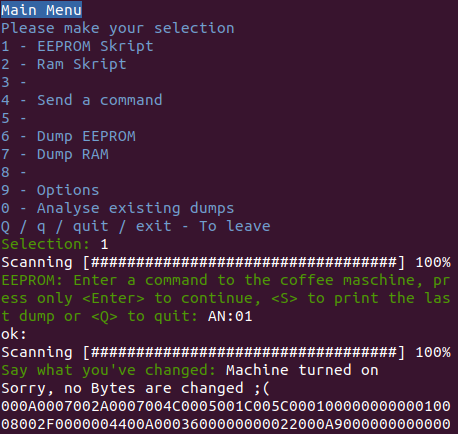
\includegraphics[scale=0.4]{images/chapter_4/JuraCoffeeMemory-3-EEPROM-NothingChanged}}\\%
%  \subfigure[Befehl senden]{\label{subfig:terminal4-Send-TY}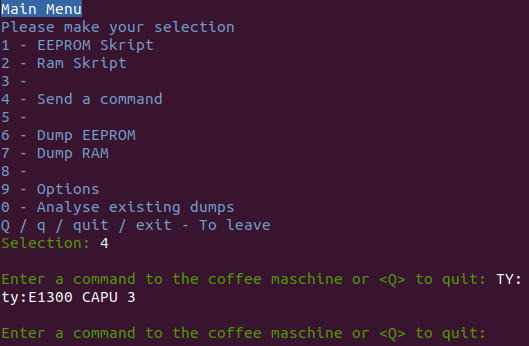
\includegraphics[scale=0.4]{images/chapter_4/JuraCoffeeMemory-4-Send-TY}}%
  \subfigure[Auswertungen]{\label{subfig:terminal8-AnalyseDumpsMenu}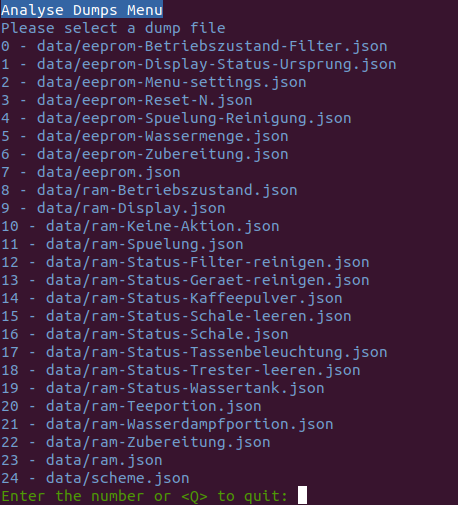
\includegraphics[scale=0.3]{images/chapter_4/JuraCoffeeMemory-8-AnalyseDumpsMenu}}\hfill%
  \subfigure[Speicherauszug einsehen]{\label{subfig:terminal9-AnalyseFilterDump}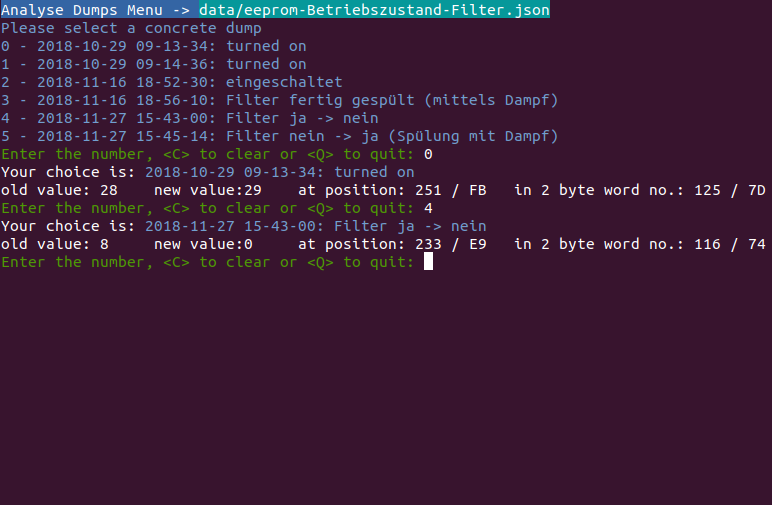
\includegraphics[scale=0.3]{images/chapter_4/JuraCoffeeMemory-9-AnalyseFilterDump}}%
}{Interaktives Menü des C++ Programms "`./JuraCoffeeMemory"'}{fig:terminal}

\begin{lstlisting}[label=lst:menu-tree,caption={Menü-Baum ./JuraCoffeeMemory}]
Main Menu
|-- 1: EEPROM Skript
|-- 2: Ram Skript
|-- 4: Send a command
|-- 6: Dump EEPROM
|-- 7: Dump RAM
|-- 9: Options
|   |-- 1: Device path (/dev/ttyACM0)
|   |-- 2: EEPROM log file path (data/eeprom.json)
|   |-- 3: Ram log file path (data/ram.json)
|   `-- 4: Back
|-- 0: Analyse existing dumps
|   |-- Analyse Dumps Menu
|   |   |-- data/xxx.json
|   |   |   `-- Dumps
|   |   |-- C: Clear window
|   |   `-- Q: Quit
|   `-- Q: Quit
`-- Q / q / quit / exit: To leave
\end{lstlisting}

\todo
Abbildung~\ref{subfig:terminal7-Options-RamLogFilePath}
Abbildung~\ref{subfig:terminal5-RAM-dump}
Abbildung~\ref{subfig:terminal3-EEPROM-NothingChanged}
Abbildung~\ref{subfig:terminal8-AnalyseDumpsMenu}
Abbildung~\ref{subfig:terminal9-AnalyseFilterDump}
\todo ...

\subsubsection{Farbcodierungen}
Normale Ausgaben sowie Benutzer Eingaben erscheinen in weißer Schrift.
Weiße Schrift auf blauem Grund stellt Menü Überschriften dar.
In blauer Schrift sind Menüs dargestellt.
Grüne Schrift vor der blinkenden Eingabemarke fordert zur Eingabe auf.
Der Text beschreibt valide Eingaben.
Abschließend beschreibt roter Text einen Fehler.
Die aufgetretene Position wird in weißer Schrift auf rotem Grund hervorgehoben.

\subsection{Die API nach außen}
Das Hauptprogramm kann aber auch über vier Parameter aufgerufen werden. Die Ausgaben sind dann im fehlerfreien Fall farblose \ac{JSON} Zeichenketten oder einfacher Text in die Standardausgabe.

Mögliche Fehlermeldungen sind für Entwickler in der \texttt{Readme.md} dokumentiert.
Die Fehler Ausgabe erfolgt wie im interaktiven Menü mit Farben.
Für Entwickler bietet sich daher der Rückgabewert des Programms an.

\paragraph{./JuraCoffeeMemory command}
Von der Standardeingabe wird eine Zeichenkette erwartet, die an den Kaffeevollautomaten weiter gegeben wird.
Mögliche Eingaben sind die Befehle aus der Tabelle~\ref{tbl:kommandos}.
Die Antwort des Kaffeevollautomaten erscheint als einfacher Text.

\paragraph{./JuraCoffeeMemory eepromWrite}
Bei diesem Aufruf wird von der Standardeingabe ein \ac{JSON} Objekt erwartet.
Alle dort genannten Bezeichnungen werden abgearbeitet und die neuen Werte im Speicher des Kaffeevollautomaten hinterlegt.
Auf der obersten Ebene müssen sich aus \texttt{EEPROM\_Status::getEntriesEEPROM()} bekannte Bezeichnungen befinden, die ein Unterobjekt mit der Bezeichnung \texttt{value} sowie je einem ganzzahligen Wert beinhalten.
Listing~\ref{lst:eepromWrite} veranschaulicht dies an einem Beispiel.

Treffen die Bedingungen zu, wird ein Schreib-Befehl an den Kaffeevollautomaten gesandt.
Die Antworten werden in einer Zeichenkette mit der verwendeten Bezeichnung und dem Text "`\#\#\#"' als Abstandshalter festgehalten und auf der Standardausgabe ausgegeben.
Die Antwort auf das Beispiel Listing~\ref{lst:eepromWrite} steht in Listing~\ref{lst:eepromWriteAnswer}.

\begin{lstlisting}[label=lst:eepromWrite,caption={Beispiel einer JSON Eingabe für./JuraCoffeeMemory eepromWrite}]
{
  "powder_quantity_special_coffee": {
    "value": 11
  },
  "water_quantity_special_coffee": {
    "value":  380
  }
}
\end{lstlisting}

\begin{lstlisting}[label=lst:eepromWriteAnswer,caption={Antwort auf das Beispiel der JSON Eingabe}]
ok: powder_quantity_special_coffee###ok: water_quantity_special_coffee###
\end{lstlisting}

\paragraph{./JuraCoffeeMemory eeprom}
Nach ungefähr fünf Sekunden erhält man die aktuellen Einstellungen und Zählstände des \ac{EEPROM} in einem kompakten \ac{JSON} Objekt.
Im Gegensatz zum EEPROM Skript werden nur die nötigen Speicherstellen abgefragt.
Die Bezeichnung der Speicherstellen, die auch der Name eines \ac{JSON} Eintrags ist, befindet sich mit der zugehörigen Adresse in \texttt{EEPROM\_Status::getEntriesEEPROM()}.
Eine Adresse besteht aus der Position eines Wortes sowie einer oder beider Bytes.
Von Hand sind dort zum Teil weitere Hintergrundinformationen, wie Standardwerte über die \texttt{[N]}-Taste des Kaffeevollautomaten, minimale und maximale Schranken, der Wert für einen deaktivierten Zustand oder überhaupt ausschließlich zugelassene Werte hinterlegt.

\paragraph{./JuraCoffeeMemory ram}
Ähnlich zum Abfragen des \ac{EEPROM} wird hier aber der \ac{RAM} in ungefähr drei Sekunden an den entscheidenden Stellen ausgelesen.
Die Assoziation einer Bezeichnung mit ihrer Speicherposition geschieht in \texttt{RAM\_Status::getEntriesRAM()}.
Hier wird ein Byte und ggf. mehrere zusammenhängende Bits als ein Eintrag abgelegt.
Als Ausgabe erfolgt ein kompaktes \ac{JSON} Objekt.










\subsection{Zugrunde liegende Klassenstruktur}

\subsection{...}\todo



% $ ll *.cpp
% EEPROM.cpp
% EEPROM_Status.cpp
% JsonFile.cpp
% JuraCoffeeMemory.cpp
% RAM.cpp
% RAM_Status.cpp
% SerialConnection.cpp
% Storage.cpp

% $ ll *.h*
% color-definitions.h
% EEPROM.hpp
% EEPROM\_Status.hpp
% JsonFile.hpp
% RAM.hpp
% RAM\_Status.hpp
% SerialConnection.hpp
% Storage.hpp

\todo

% ./RAM.cpp
% ./JsonFile.cpp
% ./Storage.cpp
% ./JuraCoffeeMemory.cpp
% ./tools/libserial-test/main.cpp
% ./tools/display.cpp
% ./tools/formate-dump.cpp
% ./tools/jsoncpp-test/main.cpp
% ./tools/display-screen-saver.cpp
% ./tools/Ideen/Ctrl-D\_stop.cpp
% ./tools/Ideen/byte-bit.cpp
% ./tools/Ideen/progressbar.cpp
% ./tools/Ideen/byte-bit-2.cpp
% ./tools/Ideen/lock-file.cpp
% ./RAM\_Status.cpp
% ./EEPROM.cpp
% ./EEPROM\_Status.cpp
% ./SerialConnection.cpp


\section{Weitere kleine Tools}\label{subsec:tools}
Im Unterordner \texttt{./tools/} befinden sich nach dem Aufruf von \texttt{make} drei kleine Programme.

\subsection{Formatieren eines Speicherauszugs}
Ruf man \texttt{./tools/formate-dump} auf, kann man dem Programm eine Zeichenkette aus $1024$ oder $512$ Hexadezimalzeichen übergeben.
Das Programm erkennt an der Größe \ac{EEPROM} und \ac{RAM} Eingaben und wertet den Speicherauszug um Angaben wie die Speicherposition und Dezimal-/Hexadezimalzahlen Formate auf.

\subsection{Display}
Um den verfügbaren Zeichensatz des Displays in der oberen linken Ecke an der Front des Kaffeevollautomaten zu bestimmen, wurde ein kleines Extraprogramm entwickelt.
Anlass waren Sonderzeichen und die deutschen Umlaute, die sich über die gegebenen Befehle (\texttt{?D0}, \texttt{?D1xxx}, \texttt{?D2xxx}) nicht einfach auf das Display bringen ließen.
Das Programm \texttt{./tools/display} iterierte einmal systematisch über die Zahlen von $0$ bis ungefähr $260$ und gab einen Befehl zum Anzeigen der Dezimalzahl sowie des dazugehörigen \ac{ASCII}-Zeichens an den Kaffeevollautomaten.
Dies umfasst das einfache und erweiterte \ac{ASCII} Alphabet sowie einige weitere Zahlen bzw. Zeichen.
Dabei stellte sich nur ein mittlerer Block des einfachen \ac{ASCII}-Alphabets als interessant heraus, der jetzt eingegrenzt von eben diesem Programm durchlaufen wird.
Ein weiteres Programm namens \texttt{./tools/display-screen-saver} veranschaulicht die damit verbundenen Möglichkeiten.

Die gegebenen Befehle über die serielle Verbindung \texttt{?D0}, \texttt{?D1xxx} und \texttt{?D2xxx} verändern nur den Standardtext "`Kaffee bereit"'.
Andere Texte, wie das Programmmenü oder Warnmeldungen, überlagern den Standardtext mit den einprogrammierten Texten aus den vorhandenen Sprachen.

Möchte man die Ausgaben des ersten Programms nachstellen ist zu beachten, dass der Kaffeevollautomat eingeschaltet sein muss und auch an die erste Displayzeile ein Ausgabebefehl gegangen ist, damit die Ausgabe auch sichtbar wird.
Das Programm verändert dann die zweite Zeile.
Folgende Befehlseingaben werden empfohlen:
\begin{enumerate}
  \item \texttt{cd JuraCoffeeMemory/}
  \item \texttt{make}
  \item \texttt{./JuraCoffeeMemory}
  \item \texttt{4} (Senden eines Kommandos)
  \item \texttt{AN:01} (Maschine einschalten)
  \item \texttt{?D1xxx} (Etwas Text an die erste Displayzeile)
  \item \texttt{<Strg>+D} (Verlassen des Programms)
  \item \texttt{./tools/display}
\end{enumerate}

\section{Die Webseite}

Die Webseite ist zu sehen in Abbildung~\ref{fig:website}.
Nach ein paar Hinweisen kann im oberen Bereich der einzelne Kaffee sowie die gesamte Maschine konfiguriert werden.
Für jede Kaffeeart ist es möglich sich seine eigene Konfiguration in einem lokalen Webbrowser-Keks (Cookie) abzuspeichern und komfortabel in den Speicher des Kaffeevollautomaten zu schreiben um sich anschließend einen Kaffee zubereiten zu lassen.
Der Keks kann auch wieder entfernt werden oder sich auf die Standardwerte zurücksetzen lassen.
Prinzipiell kann hierüber der ganze bekannte \ac{EEPROM} überschrieben werden.

Im nächsten Absatz sind Statusinformationen aus dem \ac{RAM} einsehbar.
Einige Meldungen werden am Bild des Kaffeevollautomaten visualisiert.
Der Status kann über \texttt{Refresh} aktualisiert werden.
Einfache "`ja"' oder "`nein"' Meldungen werden durch eine grünes "`on"' oder rotes "`off"' präsentiert.
Informationen, die sich über mehrere Bits erstrecken werden mit ihrem entsprechenden Zahlenwert dargestellt.

Im letzten Abschnitt befinden sich Zählstände und Prozent-Anzeigen, die verdeutlichen wie weit es noch bis zur nächsten Warnmeldung, wie Trester leeren, Maschine reinigen oder Filter wechseln, ist.

Wenn am Computer der Mauszeiger auf einer Zahl oder Einstellung zum Finger wird, öffnet sich mit einem Klick ein Fenster, in dem der Wert verändert werden kann.
Nach Möglichkeit werden der Standardwert, der Wert zum Deaktivieren und weitere Hinweis Texte angeboten.

Unten rechts auf der Seite kann über \texttt{Command} ein Kommando aus der Tabelle~\ref{tbl:kommandos} an den Kaffeevollautomaten abgesetzt werden.
Eine Liste bietet viele Vorschläge mit dazugehörigen Bezeichnungen.
Recht daneben aktualisiert ein Klick auf \texttt{Refresh} die Statusinformationen aus dem \ac{RAM}.
Ganz rechts in der Ecke kann eine Tour durch die Bedienung der Seite gestartet werden.

\begin{figure}
  \begin{center}
    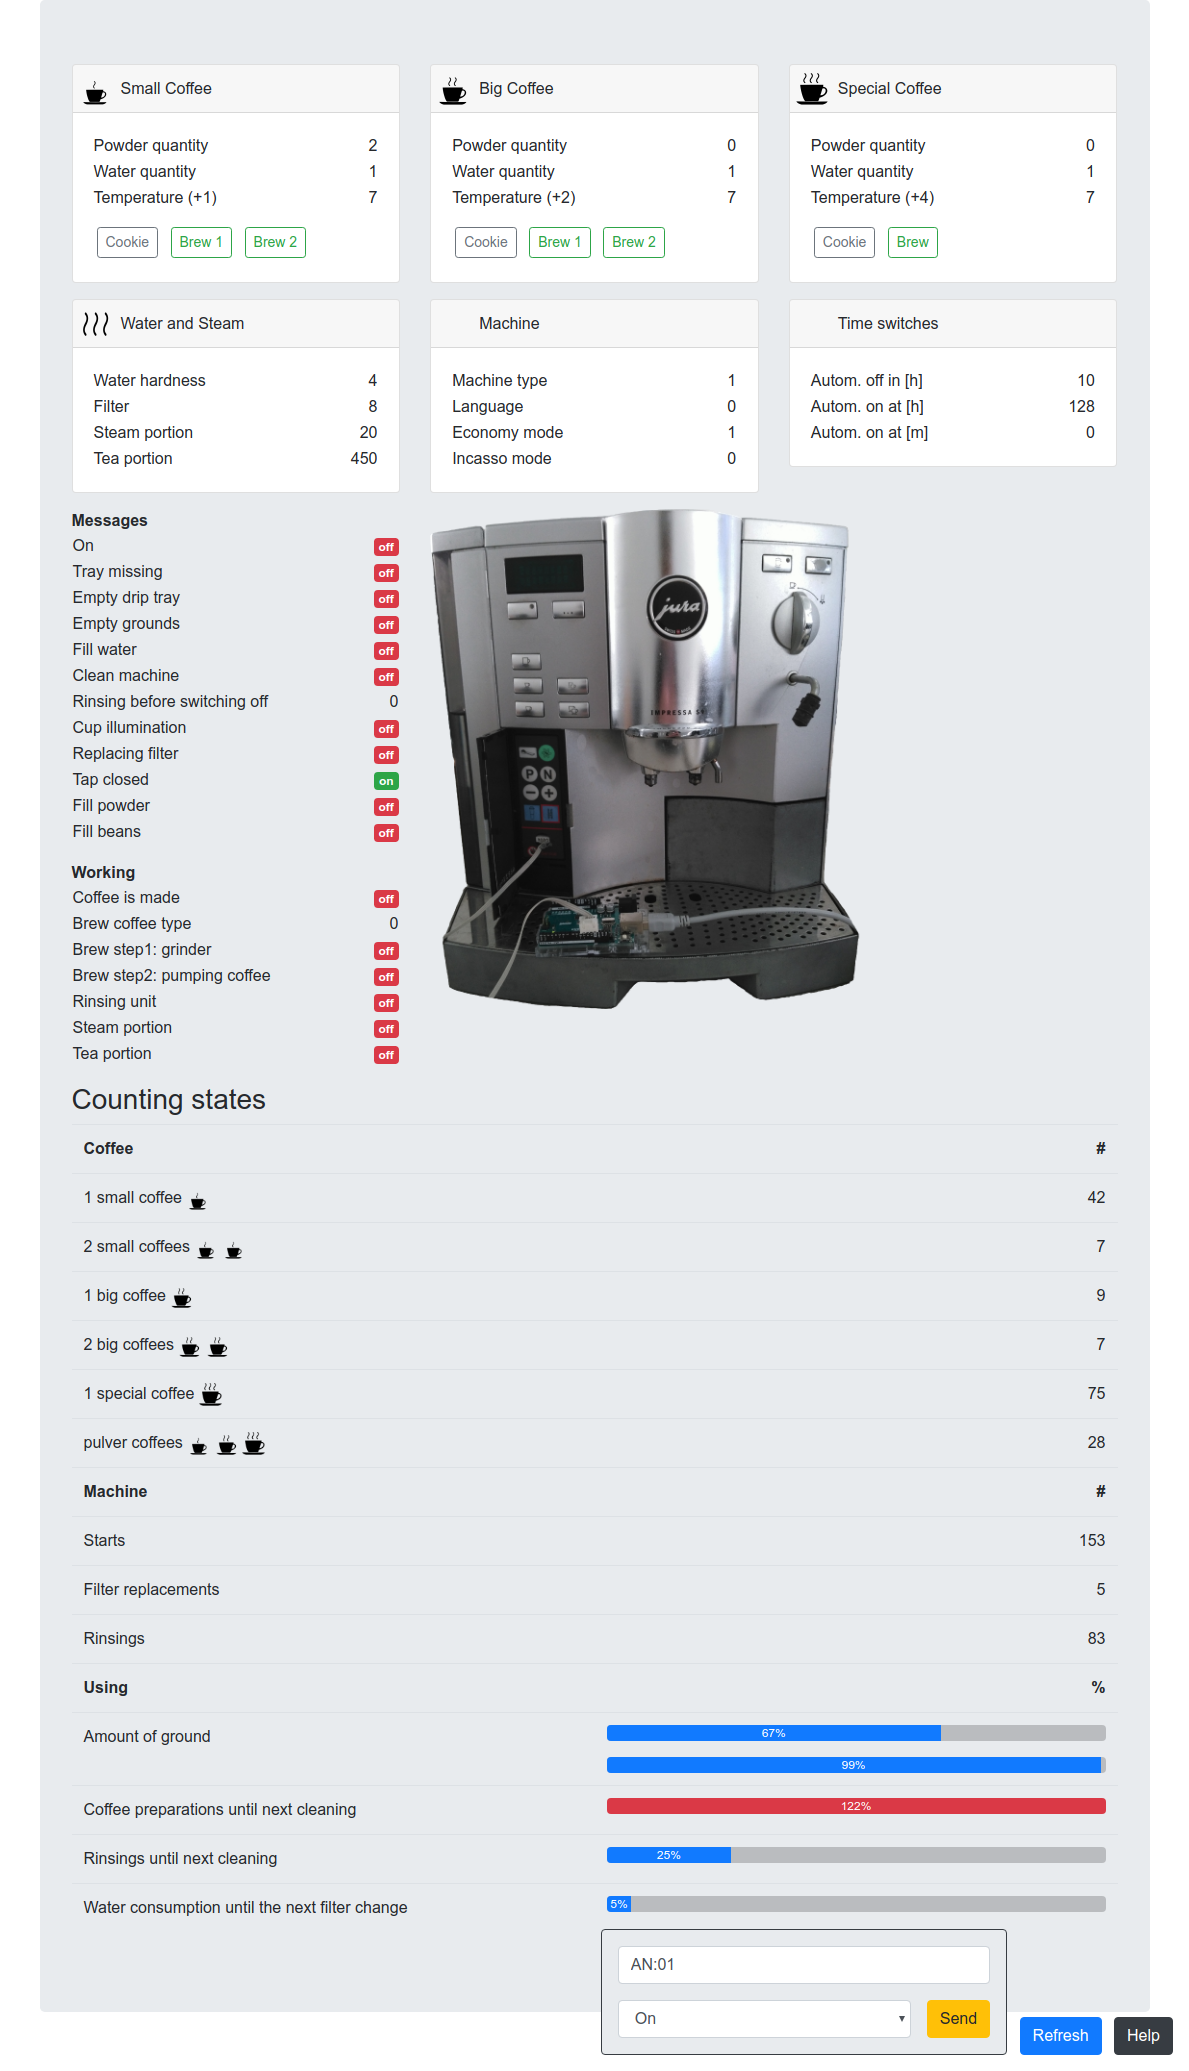
\includegraphics[scale=0.25]{images/chapter_4/Webseite}
    \caption{Die Webseite}
    \label{fig:website}
  \end{center}
\end{figure}

\subsection{Die technische Umsetzung}
Die Webseite befindet sich im Projektunterordner \texttt{./website/}.
Die Datei \texttt{data.php} nimmt Parameter entgegen und ruft damit das C++ Programm mit evtl. Datenübergaben auf.
Die Antwort des C++ Programms wird in einem \ac{JSON}-Objekt verpackt und der Webseite zurück gegeben.
Bei Problemen wird aber auch die Fehlernummer (der Rückgabewert des Programms) einschließlich der Meldung leicht zugänglich in einem \ac{JSON}-Objekt zurück gegeben.

Die für den Benutzer ersichtliche Webseite besteht primär aus den Dateien \texttt{index.html}, \texttt{script.js} für die Interaktion und \texttt{style.css} für das individuelle Layout.
Weitere eingebundene Dateien sind das Favicon im Unterordner \texttt{favicon/}, Bilder im Unterordner \texttt{img/}, \texttt{intro.min.js} und \texttt{intro.min.css} für die Tour durch die Webseite, \texttt{offline\_eeprom.json} und \texttt{offline\_ram.json} für die Offline-Funktion, in der die Webseite ersichtlich ist, ohne eine Verbindung zu dem Kaffeevollautomaten zu haben.

Das \ac{HTML} Dokument der Webseite besteht aus vielen leeren Inhaltselementen, die im Attribut \texttt{id="..."} Einträge haben, die mit den Bezeichnungen der \ac{JSON} Elemente der Ausgabe von der API des C++ Programms übereinstimmen.
Beim Seitenaufbau wird der \ac{EEPROM} abgefragt.
Wenn die Antwort nach ungefähr 5~Sekunden vorliegt wird der \ac{RAM} abgefragt und anschließend nach ungefähr weiteren 3~Sekunden für jeden \ac{JSON} Eintrag der Wert in das gleichnamige \ac{HTML} Inhaltselement eingetragen.

Eine Ausnahme bildet die Temperatur, die für alle drei Kaffeegrößen gilt, aber im Dokument drei verschiedene ID-Bezeichnungen besitzen muss.
Ebenso ist etwas Handarbeit bei der Ausgabe der Prozent-Anzeigen von Nöten.

Das bei einem Klick aufgehende Fenster zum Bearbeiten von Werten aus dem \ac{EEPROM} arbeitet ebenfalls über die ID-Bezeichnung und entnimmt weitere Informationen aus dem \ac{JSON} Objekt welches zuletzt abgefragt und abgespeichert wurde.
 % Methodik und Implementierung
\chapter{Ergebnisse}\label{ch:Ergebnisse} % Speicher / Analyse / Zusammenfassung / Ergebnisse
Die "`Jura Impressa S9"' besitzt einen \ac{RAM} für die Status, Messwerte und Zwischenberechnungen im Betrieb und einen \ac{EEPROM} für Einstellungen und Zählstände, die auch nach einer Stromunterbrechung erhalten bleiben.
Durch die Anwendung des Vorgehens in Abschnitt~\ref{sec:Vorgehen} können Aussagen zu 40 von 255 Wörtern im \ac{EEPROM} und 43 von 255 Bytes im \ac{RAM} getroffen werden.
Für den \ac{RAM} bedeutet dies 19 Statusinformationen und die Position mehrerer Zähler.

\section{EEPROM}
In Abschnitt~\ref{subsubsec:SpeicherDesKaffeevollautomatenEEPROM} wurde der vorhandene \acf{EEPROM} Speicher mit seinen 512 Bytes aufgeführt.
Im Folgenden wird vom "`Wort"', bzw. dessen ersten (XX) und zweiten (YY) Byte gesprochen.
Dabei gilt: "`Wort"' $= 256\times$"`erstes Byte"' $ + $ "`zweites Byte"' oder auch eine Antwort des Kaffeevollautomaten in der Form \texttt{re:YYXX}.

Abbildung~\ref{subfig:EEPROM} zeigt noch einmal das Speicherschema des \ac{EEPROM}.

\subsection{Kaffeezubereitung}\label{subsec:ErgebnisKaffeezubereitung}
Der Kaffeevollautomat unterscheidet bei der Zubereitung zwischen einem einmaligen Pulver-Kaffee und der normalen Zubereitung über das Bohnenfach.
Nur im Falle eines \bezeichnung{Pulver-Kaffees} wird der Zähler in Wort \wort{06} um \wert{einen inkrementiert}.
\bezeichnung{1 großer Kaffee}, \bezeichnung{2 große Kaffees}, \bezeichnung{1 kleiner Kaffee}, \bezeichnung{2 kleine Kaffees} und ein \bezeichnung{Spezialkaffee} werden bei einer Zubereitung über das Bohnenfach einzeln in den Zählern der Wörter \wort{00} bis \wort{04} in eben dieser Reihenfolge erfasst.
Der in den Einstellungen des Kaffeevollautomaten angezeigte \bezeichnung{Bezüge Zähler} gibt die Summe der bis hier genannten \wert{sechs Zähler} aus.

Die Zähler in den Worten \wort{0F} und \wort{15} werden bei \bezeichnung{jeder Zubereitung} jeweils um \wert{einen inkrementiert}, egal ob ein einfacher oder ein doppelter Bezug erfolgt, ebenso egal ob als Pulver-Kaffee oder über das Bohnenfach.
Erreicht der Wert in \wort{0F} eine Anzahl von \wert{220} Bezügen erscheint eine Reinigungsankündigung.

Darüber hinaus gibt es zwei \bezeichnung{partielle Zähler} in den Worten \wort{0D} und \wort{10}, die ungefähr bei jeder dritten Zubereitung oder Spülung um \wert{einen inkrementiert} werden.
Der genaue Grund dafür ist bisher unbekannt.

Der \bezeichnung{Trester} Stand in der Schale dieses Kaffeevollautomaten wird nicht gemessen, sondern bei jeder Zubereitung in \bezeichnung{zwei Zählern} vermerkt.
In Wort \wort{0E} ist nicht genau bekannt, wann um einen inkrementiert wird.
Ab einem Wert von \wert{16} folgt dann aber die Meldung "`Trester leeren"'.\\
Ein zweiter Trester Zähler befindet sich hinter Wort \wort{34}.
Je nach eingestellter Pulvermenge wird der Zähler um mehrere Einheiten erhöht.
Ab einem Wert von \wert{960} folgt ebenfalls die Meldung "`Trester leeren"'.\\
Beide Werte werden bei der Entnahme der Schale für mindestens 8 Sekunden automatisch auf \wert{0} zurück gesetzt.
Dies geschieht auch bei einer Reinigung.

\subsection{Kaffee Einstellungen}
Die \bezeichnung{Pulvermenge} kann in 29 Stufen auf einer Skala von \wert{0} bis \wert{28}, für einen kleinen Kaffee in Wort \wort{82}, für einen großen Kaffee in Wort \wort{83} und für einen Spezialkaffee in Wort \wort{84}, jeweils im zweiten Byte eingestellt werden.
Der Standardwert, über die \texttt{[N]}-Taste am Kaffeevollautomaten, beträgt \wert{5} für einen kleinen Kaffee, \wert{8} für einen großen Kaffee und \wert{11} für einen Spezialkaffee.
Die Menge wird automatisch für zwei kleine Kaffees und zwei große Kaffees hochgerechnet.

Die \bezeichnung{Wassermenge} eines kleinen Kaffees wird in Wort \wort{86}, eines großen Kaffees in Wort \wort{87} und eines Spezialkaffees in Wort \wort{88} über beide Bytes hinweg gespeichert.
Der Standardwert, über die \texttt{[N]}-Taste am Kaffeevollautomaten, beträgt \wert{180} für einen kleinen Kaffee, \wert{340} für einen großen Kaffee und \wert{380} für einen Spezialkaffee.
Auch hier wird die Menge automatisch auf zwei kleine Kaffees und zwei große Kaffees hochgerechnet.

Die \bezeichnung{Temperatur} kann für einen kleinen Kaffee, für einen großen Kaffee und für einen Spezialkaffee jeweils normal oder hoch eingestellt werden.
Der Standardwert liegt bei \wert{0} im zweiten Byte von Wort \wort{85} und bedeutet eine normale Temperatur für alle Sorten.
Möchte man einen kleinen Kaffee auf heiß stellen addiert man \wert{1}, für einen großen Kaffee addiert man \wert{2} und für einen Spezialkaffee addiert man \wert{4} auf den alten Wert.
Der Wert \wert{7} ist somit das Maximum und bedeutet eine heiße Temperatur für alle Sorten.

\subsection{(Tee-) Wasser- und Dampfportionen}
In Wort \wort{BB} wird die Größe einer \bezeichnung{Dampfportion} in Sekunden abgespeichert.
Nach der eingestellten Zeit endet automatisch die Dampfausgabe am Kaffeevollautomaten beim Bezug einer Dampfportion.

In Wort \wort{BC} wird die Größe einer \bezeichnung{Teeportion} abgespeichert.
Die Einheit ist hier nicht bekannte, es könnte sich aber um die Größenordnung von $0.1$ Sekunden handeln.
Wird das Drehrad von der Position "`Kaffeetasse"' auf "`Teeauslass"' gestellt wird eine Teeportion an heißem Wasser ausgegeben und automatisch beendet.

\subsection{Weitere Maschinen Einstellungen}
Wort \wort{24} speichert im ersten Byte die Information der \bezeichnung{Wasserhärte}.
Der Wert \wert{0} deaktiviert die Wasserhärte-Funktion.
Die Werte \wert{1} bis \wert{4} repräsentieren die vier Stufen, die im Benutzerhandbuch zur Maschine ausgeführt werden.
In dem zweiten Byte wird der \bezeichnung{Economy Mode} gesteuert.
\wert{1} aktiviert diesen und \wert{0} deaktiviert diesen.

In Wort \wort{25} wird die \bezeichnung{automatische Einschaltzeit} des Kaffeevollautomaten bei eingestellter Uhrzeit gespeichert.
Das erste Byte speichert die \bezeichnung{Stunde} in einem Wertebereich von \wert{0} bis \wert{23} und das zweite Byte die \bezeichnung{Minute} in einem Wertebereich von \wert{0} bis \wert{59}.
Der deaktivierte Zustand ist gegeben, wenn die Stunde auf \wert{0} und die Minute auf \wert{128} steht.

In Wort \wort{26} steht im zweiten Byte die \bezeichnung{automatische Ausschaltzeit}.
Möglich sind die Werte \wert{0}, \wert{1}, \wert{2}, \wert{4}, \wert{6}, \wert{8}, \wert{10}, \wert{12}, \wert{14}, \wert{16} und \wert{18}.
Wert \wert{0} bedeutet deaktiviert, die übrigen Werte geben ein Intervall in halben Stunden an, nach dem sich der Kaffeevollautomat automatisch abschaltet.
Das bedeutet, dass $0,5$ Stunden das Minimum und $9$ Stunden das Maximum ist.

In Wort \wort{31} befindet sich nach \cite{GitCoffeeMachine} der \bezeichnung{Maschinen Typ}.
Dieser kann mittels \texttt{RE:31} gelesen und mittels \texttt{WE:31,xxxx} überschrieben werden.

In Wort \wort{7D} befindet sich ein Zähler, der bei jedem Einschaltvorgang inkrementiert wird und somit die totale \bezeichnung{Anzahl an Einschaltvorgängen} erfasst.
Ausschaltvorgänge werden nicht vermerkt.

In Wort \wort{81} befindet sich im zweiten Byte die \bezeichnung{Spracheinstellung}.
Die folgenden Werte repräsentieren folgende Sprachen:
\wert{0} Deutsch,
\wert{16} Italienisch,
\wert{32} Niederländisch, 
\wert{48} Spanisch,
\wert{64} Englisch,
\wert{80} Französisch und
\wert{96} Portugiesisch.

In Wort \wort{B0} wird im zweiten Byte mit einem Wert von \wert{16} der \bezeichnung{Inkasso Modus} aktiviert und mit einem Wert von \wert{0} deaktiviert.
Bei eingeschaltetem Inkasso Modus erfolgt kein Bezug mehr über die Bezugstasten an der Vorderseite des Gehäuses, jedoch wird die gedrückte Taste über die \ac{UART} Schnittstelle weitergeleitet.
Mit dem entsprechenden Befehl kann über die serielle Schnittstelle dann aber die Zubereitung angestoßen werden.\\
Man erhält von dem Kaffeevollautomaten auf Knopfdruck
\texttt{?PAE} für einen kleinen Kaffe,
\texttt{?PAF} für zwei kleine Kaffees,
\texttt{?PAA} für einen großen Kaffee,
\texttt{?PAB} für zwei große Kaffees,
\texttt{?PAG} für einen Spezialkaffee,
\texttt{?PAJ} für eine Dampfportion,
\texttt{?PAI} für Wasserdampf und
\texttt{?PAK} für heißes Teewasser.

\subsection{Filter}
In Wort \wort{7D} wird im zweiten Byte gespeichert, ob ein \bezeichnung{Filter eingelegt} ist.
Der Wert \wert{0} steht für "`nein"', \wert{8} bedeutet "`ja"'.
Dieser Wert hat Einfluss auf Zähler an anderen Speicherstellen, die zum Teil nur im Falle eines "`ja"' weiter gezählt werden.

In Wort \wort{05} befindet sich ein \bezeichnung{Filter-Zähler}, der für jeden neu eingesetzten Filter inkrementiert wird.

Bei einem Filterwechsel werden die Werte in den Worten \wort{B1}, \wort{B3} und \wort{C1} (Bedeutung unbekannt) auf \wert{0} zurück gesetzt.
Erreicht der Wert in Wort \wort{B3} einen Stand von \wert{500} sind 50 Liter Wasserdurchfluss erreicht und der Filter muss gewechselt werden.
Laut Handbuch sollte ebenso spätestens nach zwei Monaten der Filter gewechselt werden.

\subsection{Spülung}
In Wort \wort{07} befindet sich ein Gesamtzähler für die \bezeichnung{Anzahl an Spülungen}.

Die partiellen Zähler hinter den Worten \wort{0D} und \wort{10} werden auch bei einer Spülung angestoßen.
Der Wert in den Worten \wort{11}, bei eingelegtem Filter auch \wort{B1} und \wort{B3}, werden bei einer Spülung um \wert{1} inkrementiert.
Erreicht der Wert in Wort \wort{B3} den Wert \wert{500} sind 50 Liter Wasserdurchfluss erreicht und der Filter muss gewechselt werden.

\subsection{Reinigung}
Die Meldung wird ausgelöst, wenn der Wert in Wort \wort{0F} einen Wert von \wert{220} erreicht hat oder der Wert in Wort \wort{11} einen Wert von \wert{180} erreicht hat.
Im ersten Fall sind 220 Bezüge erfolgt, im zweiten Fall waren es 180 Spülungen.

In den Worten \wort{07} (Anzahl an Spülungen), \wort{08} (Bedeutung unbekannt), \wort{7C} (Bedeutung unbekannt) und am Ende nach der abschließenden Spülung bei eingelegtem Filter in \wort{B1} und \wort{B3} wird der Wert um \wert{1} inkrementiert.
In den Worten \wort{10} und \wort{B3} wird der Wert um \wert{10} inkrementiert.
Die Werte in den Worten \wort{0E}, \wort{0F}, \wort{11} und \wort{34} werden zurück auf \wert{0} gesetzt.
Wort \wort{11} wird jedoch anschließend an die abschließende Spülung gleich wider um \wert{1} inkrementiert.

Wort \wort{29} Byte eins wird zu Beginn einer Reinigung auf \wert{65} gesetzt und am Ende auf \wert{0} zurück gesetzt.

\section{RAM}\label{sec:ErgebnisseRAM}
In Abschnitt~\ref{subsubsec:SpeicherDesKaffeevollautomatenRAM} wurde der vorhandene \acf{RAM} Speicher mit seinen 256 Bytes aufgeführt.
Jedes Byte besitzt acht Bits, die im Folgenden mit den Nummern 0 ($=1\times 2^0$) bis 7 ($=1\times 2^7$) bezeichnet werden.
Abbildung~\ref{subfig:RAM} zeigt noch einmal das Speicherschema des \ac{RAM}.

Aufgrund starker, aber zum Teil regelmäßiger Schwankungen, wurden die folgenden Bytes über mehrere Speicherauszüge ohne zwischenzeitliche Veränderungen ermittelt und \bezeichnung{für diese Arbeit ausgeblendet}:
\wort{02}, \wort{09}, \wort{0C}, \wort{1C} bis \wort{21}, \wort{27}, \wort{28}, \wort{2A}, \wort{2C}, \wort{2E}, \wort{41}, \wort{66}, \wort{67}, \wort{6A}, \wort{6C}, \wort{70}, \wort{7C}, \wort{94}, \wort{95}, \wort{97}, \wort{9C}, \wort{9D}, \wort{A2}, \wort{F1} und \wort{FC} bis \wort{FF}.

Die Aufschlüsselung und der Bezugspunkt für die im Folgenden genannten Rubriken sind die Spalten der Tabelle~\ref{tbl:RAM1} und der Tabelle~\ref{tbl:RAM2}.

Unterstrichene und hervorgehobene Zellen sind "`immer"' abfragbar.
Die einzige Voraussetzung ist die in Abschnitt \ref{subsec:AufbauUndVerkabelung} beschriebene Verkabelung, sowie eine angelegte Netzspannung an den Kaffeevollautomaten.
Der Kaffeevollautomat \underline{muss} sich dann \underline{nicht} im eingeschalteten Zustand befinden.

Eingeklammerte Zellen haben sind nicht exklusiv für die genannte Rubrik, sie teilen sich den Wert mit weiteren Funktionen.

\subsection{Maschine an}
Sobald der Kaffeevollautomat eingeschaltet wird ändern sich die Werte mehrerer Speicherstellen im \ac{RAM}.
Tabelle~\ref{tbl:RAM1} zeigt die regelmäßigen Änderungen beim Einschalten in der ersten Spalte "`Maschine an"'.
Der Umschwung der sieben Bits erfolgt sofort nach der Betätigung des "`Ein"'-Schalters, selbst wenn sich der Kaffeevollautomat noch aufwärmt und "`Bitte warten"' anzeigt.
Eine Änderung nach der Aufwärmphase konnte nicht festgestellt werden.

Beim Ausschaltet geschehen die Änderungen umgekehrt.

\subsection{Schale fehlt}
Die beiden linken Kontakte, die eine eingesetzte Schale verbindet, sind voneinander getrennt.
Ohne eine eingesetzte Schale schaltet der Kaffeevollautomat sicherheitshalber alle Tätigkeiten ab.
Dies wird auch im ausgeschalteten Zustand vermerkt.

Die Änderungen sind in Tabelle~\ref{tbl:RAM1} in der zweiten Spalte dargestellt.
In \bytebit{16}{0} und in \bytebit{69}{0} steht nur eine \wert{0}, wenn der Kaffeevollautomat eingeschaltet ist.
Die an anderen beiden Bits enthalten zu jeder Zeit den aktuellen Status.

\subsection{Schale leeren}
Die linken beiden und der rechte Kontakt sind kurzgeschlossen.
Der Wasserstand in der Auffangschale ist dann gefährlich hoch und der Kaffeevollautomat schaltet sicherheitshalber alle Tätigkeiten ab.
Dies wird auch im ausgeschalteten Zustand vermerkt.

Die Änderungen sind in Tabelle~\ref{tbl:RAM1} in der dritten Spalte dargestellt.

\subsection{Trester leeren}
Hat einer der beiden Trester Zähler seine Grenze erreicht, erfolgt die Aufforderung den Trester zu leeren.
Indem die Schale für mindestens acht Sekunden entnommen wird, werden beide Zähler auf \wert{0} zurück gesetzt.

Eine wichtige Ergänzung zur Tabelle~\ref{tbl:RAM1} ist, dass nur der Trester Zähler im \ac{EEPROM} in Wort \wort{34} die Änderung im \ac{RAM} in \bytebits{80}{1}{0} auslöst.
Um allgemein diese Meldung ausschließen zu können muss sich der Kaffeevollautomat im eingeschalteten Zustand befinden.

\subsection{Wasser füllen} % Wassertank entnommen
Bei dieser Meldung schließt der magnetische Schwimmer im Wassertank nicht den Kontakt und die Meldung leuchtet auf.
Der Wasserspiegel kann hierbei zu niedrig sein oder der Wassertank wurde zum Auffüllen oder Wasser Wechseln entnommen.
Dies wird auch im ausgeschalteten Zustand vermerkt.

Die Änderungen sind in Tabelle~\ref{tbl:RAM1} in der fünften Spalte dargestellt.

\subsection{Gerät reinigen}
Sind 220 Bezüge oder 180 Spülungen erreicht, wird eine Reinigung gefordert.
In \bytebit{10}{7} und in \bytebit{22}{4} steht dann je eine \wert{1}, siehe Tabelle~\ref{tbl:RAM1} Spalte sechs.

\subsection{Maschine spült}
Wenn der Kaffeevollautomat eine Spülung vornimmt wird dies in mehreren Bits vermerkt.
Die Änderungen sind in Tabelle~\ref{tbl:RAM1} in der siebten Spalte dargestellt.

\subsection{Maschine vor dem Ausschalten spülen}
Der Kaffeevollautomat erzwingt eine Spülung vor dem Ausschalten, wenn während der Betriebszeit ein Kaffeebezug erfolgte, ohne eine abschließende Spülung vorgenommen zu haben.
In \bytebits{0D}{3}{2} steht in diesem Fall mal an dem einen und mal an dem anderen Bit eine \wert{1}.
Dieser Merker befindet sich sehr wahrscheinlich hier, auch wenn die genau Bedeutung der einzelnen Bits nicht sicher bekannt ist.

\subsection{Tassenbeleuchtung}
Bei einer Zubereitung oder laut Benutzerhandbuch auch durch das Drücken einer beliebigen Taste im ausgeschalteten Zustand wird die Tassenbeleuchtung eingeschaltet.
Nach drei Minuten schaltet die Tassenbeleuchtung dann wieder automatisch ab.

In \bytebitss{0F}{2}{1} steht bei eingeschalteter Tassenbeleuchtung "`immer"' mindestens eine \wert{1}.
Beim Betreten des Menüs oder auch beim Ausschalten wird mindestens eine \wert{1} gesetzt.
Eine genaue Aufschlüsselung oder Zuordnung der beiden Bits zu bestimmen Rahmenbedingungen konnte nicht hergestellt werden.

\subsection{Filter wechseln}
Ist ein Durchfluss von 50 Litern erfolgt, erscheint diese Meldung mit der Aufforderung den Wasserfilter auszuwechseln.
Die Änderungen sind in Tabelle~\ref{tbl:RAM2} in der ersten Spalte dargestellt.
Diese Meldungen kann im ausgeschalteten Zustand des Kaffeevollautomaten abgefragt werden.

\subsection{Hahn offen \& Teeportion}
Wird der Drehknauf von der "`Kaffeetasse"' weg gedreht, wird der \bezeichnung{Hahn geöffnet}.
Erreicht der Regler darüber hinaus die Stellung des "`hinplätschernden Wasserhahns"', ist eine \bezeichnung{Teeportion} aktiv.

Die Änderungen sind in Tabelle~\ref{tbl:RAM2} in der zweiten und dritten Spalte dargestellt.
Auch diese Meldungen können im ausgeschalteten Zustand des Kaffeevollautomaten abgefragt werden.

\subsection{Dampfbezug \& Wasserdampfportion}
Beim \bezeichnung{Dampfbezug} wird bis zur erneuten Betätigung der Taste heißer Wasserdampf aus dem rechten Rohr ausgegeben.
Eine \bezeichnung{Wasserdampfportion} ist zeitlich begrenzt und kann in den Einstellungen dimensioniert werden.

Die Änderungen sind in Tabelle~\ref{tbl:RAM2} in der vierten und fünften Spalte dargestellt.
Die einzige Position für eine sichere Unterscheidung ist in \bytebit{13}{1}, wo nur bei dem Dampfbezug eine \wert{1} steht.

\subsection{Pulver füllen}
Hinter der Wartungsklappe befindet sich die Wahltaste für vorgemahlenes Kaffeepulver.
Wird diese betätigt, wird der nächste Kaffeebezug einmalig über das Pulverfach zubereitet und es werden keine Bohnen gemahlen.
Dieser Modus kann ebenfalls über die serielle \ac{UART} Schnittstelle mit dem Befehl \texttt{FA:03} ausgelöst werden.

In \bytebit{04}{0} befindet sich dann eine \wert{1}, die nach dem nächsten Bezug automatisch wieder auf \wert{0} zurück gesetzt wird.

\subsection{Bohnen füllen}
In \bytebit{0E}{7} steht eine \wert{1} im Falle fehlender oder verklemmter Bohnen.
Die Meldung verschwindet mit ausreichend Bohnen im Steinchen losen Bohnenfach beim nächsten Bezug.

\subsection{Zubereitung}\label{subsec:RAM:Zubereitung} % -> Aktionsauswirkungen?!
Für eine Kaffeezubereitung werden im \bezeichnung{ersten Schritt} die Bohnen gemahlen.
In \bytebits{03}{7}{4} steht dann je eine \wert{1}.
In \bytebit{03}{7} steht nur während einer Kaffeezubereitung eine \wert{1} und nicht im Falle des manuellen Starts des Mahlwerks mit dem Befehl \texttt{FN:07} oder \texttt{FN:09}.

Im \bezeichnung{zweiten Schritt} wird der Kaffee Aufgebrüht und Ausgeschenkt.
Die Änderungen sind in Tabelle~\ref{tbl:RAM2} in der letzten Spalte dargestellt.

Über die \bezeichnung{gesamte Zeit} steht in \bytebit{0A}{6} eine \wert{1}.
Darüber hinaus steht in \bytebitss{0A}{2}{0} die gewählte Portion kodiert.
\wert{1} steht für einen kleinen Kaffee, \wert{2} steht für 2 kleine Kaffees, \wert{3} steht für einen großen Kaffee, \wert{4} steht für 2 große Kaffees und \wert{5} steht für einen Spezialkaffee.

\subsection{Geteilte Bits}
In Tabelle~\ref{tbl:RAM1} und Tabelle~\ref{tbl:RAM2} sind mehrere Einträge eingeklammerte.
Im Folgenden sollen einige Zusammenhänge gegenüber gestellt werden:

In \bytebits{03}{6}{1} steht der Wert auf \wert{1}, wenn der Kaffeevollautomat eine Spülung vornimmt, eine Teeportion ausschenkt oder sich manchmal in der Zubereitung eines Kaffees befindet.
In \bytebit{03}{6} war gerade die Zubereitung unregelmäßig, während sich \bytebit{03}{1} reproduzierbar verhielt.
Auch in \bytebit{62}{1} steht eine \wert{1} und in \bytebit{68}{5} steht eine \wert{0} wenn die Maschine spült oder sich im zweiten Schritt der Zubereitung befindet.
In \bytebit{68}{6} steht eine \wert{1}, wenn eine Teeportion ausgegeben wird oder die Maschine spült.

In \bytebits{03}{3} kommen eine Wasserdampfportion sowie das Einschalten direkt nach dem Ausschalten mit abschließender Spülung zusammen.

In \bytebit{04}{3} steht eine \wert{1}, wenn die Schale fehlt, der Wassertank fehlt oder die Schale voll ist, aber auch beim offenen Hahn oder dem Dampfbezug.

In \bytebit{04}{3} steht eine \wert{0} bei einer Teeportion, beim Dampfbezug, bei einer Wasserdampfportion oder auch bei der Zubereitung eines Kaffees.
In \bytebit{4C}{0} steht eine \wert{0} beim Wasser füllen oder offenem Hahn.
Auch in \bytebit{91}{0} steht eine \wert{0} beim Wasser füllen aber wechselhaft bei der Zubereitung eines Kaffees.

In \bytebit{16}{0} und \bytebit{69}{0} steht eine \wert{0}, wenn die Schale fehlt oder die Maschine aus ist, andernfalls befindet sich der Kaffeevollautomat hier in einem betriebsbereiten Zustand.

\subsection{Deutung und Zähler}
Im \ac{RAM} könnte \bytebitss{13}{2}{0} für eine interne Wasserschaltung stehen.

In den Bytes \wort{37} bis \wort{3C}, in Byte \wort{43}, sowie in den Bytes \wort{71} bis \wort{75} befinden sich sehr wahrscheinlich interne Zählstände, die während einer Kaffeezubereitung oder allgemeiner beim Pumpen von Wasser rauf zählen.
In dem Byte \wort{8B} sowie bis in das davor liegende Byte \wort{8A} reicht eine Zähler für primär den Dampfbezug oder eine Wasserdampfportion, aber auch bei einer Kaffeezubereitung oder Spülung bewegt sich der Zähler.

\section{Alleinstellungsmerkmal für die API und die Webseite}
Tabelle~\ref{tbl:RAM1} und Tabelle~\ref{tbl:RAM2} machen deutlich, dass es mehrfach redundante Speicherstellen im \ac{RAM} gibt an potentiell denen die gleiche Information steht.
Da die serielle Übertragung abgefragter Speicherstellen Zeit benötigt, versucht die \ac{API} nur die wirklich nötigen Speicherstellen abzufragen und dadurch Zeit einzusparen.

Abbildung~\ref{fig:API-EEPROM} zeigt die abgefragte Speicherstellen für die \ac{API} im \ac{EEPROM}.
Es werden vier Zeilen und drei einzelne Worte abgefragt.
Da auch die Anfrage in der Übertragung Zeit benötigt, ist eine Zeile effizienter als sechzehn einzelne Wörter.

Abbildung~\ref{fig:API-RAM} zeigt die abgefragte Speicherstellen für die \ac{API} im \ac{RAM}.
Hier können nur ganze Zeilen abgefragt werden, aber diese können an beliebiger Stelle beginnen.
Es reichen für alle Funktionen vier Zeilen aus.
Viele interne Zähler und Dopplungen können ausgelassen werden.
Dennoch wird deutlich, dass die Bytes bestimmter Statusinformationen, die an verschiedenen Bits stehen, sehr nahe beieinander liegen und an anderer Stelle einzelner Bytes effizienter als ganze Reihen wären.

\section{Display}\label{sec:Display}
Das Display der "`Jura Impressa S9"' umfasst zwei Zeilen mit je acht Zeichen, die wiederum mit je $5 \times 5$ Lichtpunkten dargestellt werden.
Tabelle~\ref{tbl:Displaysymbole} zeigt die verfügbaren Schriftzeichen auf.
Es handelt sich um arabische Zahlen, große lateinische Buchstaben sowie ein paar Sonderzeichen, die unter anderem eine Skala darstellen können.

$0_{10}$ bis $31_{10}$ und alle \ac{ASCII}-Zeichen über $97_{10}$, auch aus der erweiterten \ac{ASCII}-Tabelle von $128_{10}$ bis $255_{10}$ und darüber, stellt der Kaffeevollautomat nicht mehr als eindeutig bekannte \ac{ASCII}-Zeichen dar.
Es handelt sich höchstens um verpixeltes Kanji und wurde in der Tabelle ausgelassen.
 % Speicher                     % Analyse / Zusammenfassung / Ergebnisse
\chapter{Diskussion}\label{ch:Diskussion}
Dieses Kapitel benennt aufgetretene Probleme während der Arbeit und hinterfragt die Ergebnisse aus dem vorherigen Kapitel.
Auch der Begriff des \textit{Reverse Engineering} wird hier wieder aufgegriffen.

\section{Probleme}
Nicht nur die Kommunikation mit dem Kaffeevollautomaten, sondern auch das Verständnis der Vorgänge in der Maschine erfordern Zeit und Arbeit.

\subsection{Kommunikation mit dem Kaffeevollautomaten} \label{subsec:zugangSeriellDirekt}
Der direkte Zugang ist wahrscheinlich am schnellsten, im laufenden Betrieb aber schlecht möglich, da die Speicheradressen aktiv abgefragt werden müssten und damit Kurzschlüsse in der Elektronik produziert werden würden.
Die serielle \ac{UART} Schnittstelle ermöglicht das Abfragen im laufenden Betrieb, also auch im \ac{RAM}.
Das Auslesen benötigt jedoch seine Zeit, ungefähr 9 Sekunden für den gesamten \ac{RAM} und ungefähr 15 Sekunden für den gesamten \ac{EEPROM}.
Gerade im \ac{RAM} gibt es viele Veränderungen im Ruhezustand, sodass auf diesem Weg nie ein zusammenhängender Speicherauszug zu einem festen Zeitpunkt ausgelesen werden kann.

Ein weiterer Nachteil ist, dass während einer Übertragung das interne Bus System gehemmt ist.
Eingaben an der Maschine, wie die Navigation durch das Menü, werden während der Erstellung eines Speicherauszugs verzögert umgesetzt.
Aber auch in der Gegenrichtung sorgen wechselnde Displaytexte für Verzögerungen während der seriellen Übertragung.

Durch die Optimierung für die \ac{API} benötigt das Auslesen nur noch ungefähr 3 Sekunden für den \ac{RAM} und ungefähr 5 Sekunden für den \ac{EEPROM}.
Abbildung~\ref{fig:API-EEPROM} und Abbildung~\ref{fig:API-RAM} zeigen die dabei abgefragten Speicherstellen.

\subsection{Serielle Kommunikation} \label{subsec:kommunikationGeraetedateiLibserialLibrary}
\paragraph{Gerätedatei direkt ansprechen}
Um mit dem Arduino und letztlich dem Kaffeevollautomaten zu kommunizieren, war der erste Versuch den Dateideskriptor \texttt{/dev/ttyACM0} sowohl lesend als auch schreibend zu nutzen.
Zunächst funktionierte dies sehr gut, bis nach wenigen Tagen kaum reproduzierbares Fehlverhalten auftrat.
Gerade Antworten der Kaffeemaschine kamen nur noch in Bruchstücken an.
Dies wurde bei der Einrichtung bereits im Projekt "`CoffeeMachine"'\cite{GitCoffeeMachine} in der \texttt{Readme.md} für die Ausführung auf einem Raspberry Pi beschrieben.

Versuche, dies direkt zu lösen, indem eine funktionierende Umgebung nachgebaut wurde, schlugen fehl.
Dabei konnte über \texttt{screen /dev/ttyACM0 9600} und \texttt{exit} die serielle Verbindung initiiert werden.
Die Einstellungen können dann über \texttt{stty -F /dev/ttyACM0} eingesehen werden, jedoch hatte es nicht denselben Effekt, nur diese Einstellungen gezielt über den Befehl
\begin{lstlisting}[label=lst:stty,caption={stty zum setzen der Verbindungseinstellungen}]
stty -F /dev/ttyACM0 9600 raw \
ignbrk -brkint -icrnl -imaxbel \
-opost -onlcr \
-isig -icanon -iexten -echo -echoe -echok -echoctl -echoke
\end{lstlisting}
zu setzen.

\paragraph{C++ und die \textit{libserial}-Library}
Für eine sichere Verbindung wird in dem C++ Programm auf die im Linux Repository erhältliche Library \textit{libserial} zurückgegriffen.
Beim Verbindungsaufbau über die \textit{connect()} Methode der \textit{SerialConnection} Klasse wird die Schnittstelle initialisiert.
Hier werden der Gerätepfad, die Baudrate und eine erwartete Mindestlänge festgelegt.

Kommandos gehen zuverlässig an den Arduino raus und ausgelesene Antworten kommen nun im Ganzen an.
Der \textit{read} Befehl ist ein blockierender Aufruf, der das Programm anhält bis eine Antwort vorliegt.
Dies stellt für die Speicherauslesung kein Problem dar, da die ordnungsgemäßen Befehle immer ein \texttt{ok:} oder \texttt{xx:0-F} Speicherauszug zurückgeben.

\subsection{Unbekannte Speicherorte}\label{subsec:UnbekannteSpeicherorte}
Bis auf den Speicherort des veränderbaren Standardtextes konnten alle Einstellungen und Grenzwerte sowie ein paar Funktionsabläufe festen Speicherstellen zugeordnet werden.
Da der Standardtext eine Stromunterbrechung nicht übersteht, liegt er sehr wahrscheinlich im \ac{RAM} oder einem weiteren flüchtigen Speicher der Maschine.
Selbst unter der Annahme, dass die Maschine vielleicht nur die halbe \ac{ASCII}-Tabelle pro Zeichen benutzt und dadurch zwei Displayzeichen pro Byte kodiert, konnten einfache und monotone Texte wie \texttt{AAAAAAAA} nicht in einem Speicherauszug wiedergefunden werden.

Um dies weiter zu ergründen, muss künftig ein Blick in die Maschine erfolgen, um die vorhandenen Speicher und deren Größen zu bestimmen.
Nach dem Datenblatt des Mikrocontrollers \cite{JuraMicrocontroller} gibt es vier Ausführungen, von der aber keine den 256 Byte \ac{RAM} und 512 Byte (256 Wörter) \ac{EEPROM}, die über die seriellen Befehle adressierbar sind, entspricht.

Es wäre vorstellbar, dass die gegebenen Befehle aus Tabelle~\ref{tbl:kommandos} nicht den insgesamt zur Verfügung stehenden Speicher adressieren und nach außen kommunizieren.
Andererseits ist es ebenfalls möglich, dass viele unbekannte Speicherstellen gar keine Funktion besitzen;
der vorhandene Speicher dieses Standard Mikrocontrollers würde von dem Programm dann nicht voll ausgenutzt werden.

\subsection{Weitere Automatisierung durch das C++ Programm}
Für den \ac{EEPROM} ist es ein vertretbarer Aufwand, Einstellungen am Gerät vorzunehmen, das Skript anzustoßen und einen Kommentar zu hinterlegen.
Die Ergebnisse können aus der \ac{JSON} Datei abgelesen werden.

Die wechselhaften Sprünge im \ac{RAM} erforderten ein wiederholtes Anwenden des Skripts, wie in Abschnitt~\ref{sec:Vorgehen} beschrieben.
Hier könnte das C++ Programm dahingehend ausgebaut werden, $n=3$ Durchläufe mit dem selben Kommentar zu versehen.
Die Auswertung sollte aber von Hand erfolgen und es sollten Ergebnisse aus variierenden Umgebungsbedingungen einbezogen werden.
Zum Beispiel den Wasserfilter einmal aktivieren und einmal deaktivieren.
Es bedürfte einer sehr guten künstlichen Intelligenz, diese Umgebungen vorzuschlagen und die Ergebnisse zusammenzuführen.

Mit dem in Abschnitt~\ref{sec:Vorgehen} beschrieben ersten Vorgehen lassen sich Statusinformationen und Einstellmöglichkeiten sehr gut auslesen.
Bedingte Abhängigkeiten, wie die Zusammensetzung eines Bezüge-Zählers aus mehreren Zählern, oder Abläufe, wie die zwei Schritte einer Kaffeezubereitung, wären durch ein starr hochgezogenes Computerprogramm unentdeckt geblieben.

Ausbaufähig ist die wieder bessere Trennung des \ac{EEPROM}s und des \ac{RAM}s.
In den gefundenen Unterschieden des Skripts können weniger relevante Spalten ausgeblendet werden und es könnten die \ac{JSON} Dateien mit einem Merker versehen werden, um der nachträglichen \textit{Aufschlüsselung der Veränderungen} im C++ Programm eine bessere Differenzierung zu ermöglichen.
Zur Zeit muss für den \ac{RAM} von Hand die Zeile 192 der \texttt{JuraCoffeeMemory.cpp} einkommentiert werden.

\section{Aussagekraft der Ergebnisse}\label{sec:AussagekraftDerErgebnisse}
Die \ac{EEPROM} Einstellmöglichkeiten können recht sicher festen Speicherstellen zugeordnet werden.
Bei einigen partiellen Zubereitungszählern ist aber nicht bekannt, wann sie zählen und wofür.
Die Firmware fehlt an dieser Stelle.

Im \ac{RAM} sind mehrere Status Bits einigermaßen aussagekräftig, vor allem aber die im ausgeschalteten Betriebszustand, die auch in Tabelle~\ref{tbl:RAM1} und Tabelle~\ref{tbl:RAM2} hervorgehoben sind.
Durch viele unregelmäßige Veränderungen wurden aber mehrere Bytes außer Acht gelassen, die an bestimmten Bit Positionen wichtige Merker enthalten könnten.

Unsicherheit besteht durch mehrere Speicherpositionen für ein und dieselbe Funktion.
Entweder verbirgt sich hinter einzelnen Positionen noch eine andere Bedeutung oder eine bisher unbekannte Abhängigkeit für weitere Funktionen.
Zustände könnten im \ac{RAM} tatsächlich mehrfach erfasst werden.

\section{Einordnung zur Terminologie des Reverse Engineerings}\label{sec:DiskussionBegriffReverseEngineering}
Diese Arbeit besteht im Wesentlichen aus den zwei Teilen, den Speicher zu analysieren und zu verstehen, bzw. das Wissen darüber in einer neuen Oberfläche einfach zur Verfügung zu stellen.
Ein kurzer Rückblick in Abschnitt~\ref{sec:Begrifflichkeiten} erinnert an die Begriffe \textit{Forward Engineering}, \textit{Reverse Engineering}, \textit{Redocumentation}, \textit{Design Recovery}, \textit{Restructuring} und \textit{Reengineering}.

Für den ersten Teil wurden eine gegebene serielle Schnittstelle und bereits implementierte Befehle ausgenutzt, um den Speicher auszulesen.
Viele Aufnahmen, mit kleinen Veränderungen zwischendurch, ließen Rückschlüsse auf die Bedeutung der Werte an bestimmten Speicherstellen zu.
Gerade mit den Überlegungen, was während einer Aktion am Kaffeevollautomaten alles im Speicher passiert, lässt sich diese Tätigkeit dem Begriff \textit{Reverse Engineering} zuordnen.
Aus dem fertig implementierten und gegebenen System werden Rückschlüsse auf das Design der Maschine gezogen.
\textit{Redocumentation} trifft aufgrund fehlender Spezifikationen und Quellcodeauszügen wenig zu.
Betrachtet man aber das Benutzerhandbuch und Interneteinträge über Erfahrungen mit der Maschine als externe Informationen, sowie Schlussfolgerungen und Unschärfelogik über den \ac{RAM}, kann dieser Part auch als \textit{Design Recovery} über den Speicher angesehen werden.

Mit diesem Wissen des ersten Teils wurde dann im zweiten Teil etwas Neues geschaffen.
Das Abfragen der aktuellen Einstellungen und Zustände bietet eine neue Oberfläche, die als \textit{Redocumentation} oder \textit{Restructuring} angesehen werden kann.
Für die \textit{Redocumentation} spricht das neue Ausgabeformat auf der Ebene der Implementierung.
Ein eigenes Gerät ist zur Alternative (Ausnahmen siehe~\ref{FehlendeMeldungen}) für das kleine Display des Geräts geworden und gibt den aktuellen Zustand in ausführlicherer Weise aus.
Ohne eine präventive Instandhaltung beabsichtigt zu haben ist \textit{Restructuring} aber auch zutreffend, da Wissen aus dem ersten Teil hier eingeflossen ist.
Wenn die Bedeutung bestimmter Speicherstellen nicht bekannt gewesen wäre, hätten die eingestellten Werte keine Bedeutung gehabt, was für den Begriff \textit{Restructuring} spricht.

Für eine individuelle Zubereitung wird nur die Datengrundlage kurz zuvor mit einem Impuls von außen verändert, der Kaffee wird dabei nach wie vor von den Standard Abläufen der Kaffeemaschine zubereitet.
Die neue Oberfläche kann als \textit{Restructuring} oder dem allgemeineren \textit{Reengineering} angesehen werden.
Da die neue Oberfläche über die serielle Schnittstelle in Verbindung mit einem eigenen Endgerät aber sehr von den Bordmitteln der Maschine abweicht, passt vielleicht das \textit{Reengineering} etwas besser.
Die Funktionalitäten der Maschine sind aber immer noch die Gleichen, das Programmmenü muss nun jedoch nicht mehr verwendet werden, um die allgemeinen Geräteeinstellungen für den eigenen Kaffee anzupassen.

Im Detail ist die genaue Zuordnung der Begrifflichkeiten immer eine persönliche Auslegung dieser Begriffe.
Sehr zutreffend ist das Zitat aus Abschnitt~\ref{sec:Begrifflichkeiten}, denn diese Arbeit hat den Speicher intensiv betrachtet und mittels der Ergebnisse aus dem zweiten Teil um neue Perspektiven bereichert, ohne das Ziel verfolgt zu haben, die Maschine zu klonen oder umzubauen.
 % Diskussion und Ausblick

% Bibliography
% if you have cited papers that are not referenced, but important for your work,
% uncommented the following line; however, this should generally by unnecessary
% and hints at improper citing.
%\nocite{*}
\tuhhbibliography{thesis}


% Appendix
% Feel free to add additional appendix chapters (e.g., measurement setups, etc.)
\begin{tuhhappendix}
  \chapter{Große Abbildungen}
Im Folgenden sind größere Abbildungen dargestellt, die eine ganze Seite oder eine Doppelseite einnehmen.

\noindent Tabelle~\ref{tbl:kommandos} führt eine Auswahl der möglichen Befehle für den Kaffeevollautomaten auf.
Die vollständige Liste befindet sich unter \texttt{JuraCoffeeMemory/result/commands.txt}.

\noindent Abbildung~\ref{fig:Speicherschema} zeigt schematisch den Speicher des Kaffeevollautomaten.
Der \ac{EEPROM} und der \ac{RAM} sind in jeweils 16 Zeilen zeilenweise dargestellt.

\noindent Tabelle~\ref{tbl:RAM1} und Tabelle~\ref{tbl:RAM2} stellen spaltenweise die Bit-Änderungen für je eine Meldung oder Funktion im \ac{RAM} dar.

\noindent Abbildung~\ref{fig:API-EEPROM} und Abbildung~\ref{fig:API-RAM} zeigen die abgefragten Wörter und Bytes für die Ausgabe der \ac{API}.

\noindent Tabelle~\ref{tbl:Displaysymbole} stellt den verfügbare Zeichensatz für das Display dar.
Gleichzeitig werden die dafür nötigen \ac{ASCII} Kommando-Eingaben aufgeführt.

\begin{tuhhtable}
  \footnotesize\centering
  \begin{tabular}[tp]{L{.22\textwidth}L{.48\textwidth}L{.18\textwidth}}
%
  \THc{1}{c}{Kommando} & \THc{1}{c}{Beschreibung} & \THc{1}{c}{Rückgabewert} \\
%
  \TRx{3}{l}{Betriebszustand (AN:<id>)}\\
  \abovebodyrule
  AN:01    & Einschalten        & ok:    \\\TRc
  AN:02    & Ausschalten        & ok:    \\
  AN:03    & Display Test       & ok:    \\\TRc
  AN:<id>  & u.v.m.             & ok:    \\
  \belowbodyrule
%
  \TRx{3}{l}{Bezugstaste (FA:<id>)}\\
  \abovebodyrule
  FA:02    & Gerät spülen       & ok:    \\\TRc
  FA:0C    & Spezialkaffee      & ok:    \\
  FA:<id>  & u.v.m.             & ok:    \\\TRc
  \belowbodyrule
%
  \TRx{3}{l}{Steuerungskomponenten (FN:<id>)}\\
  \abovebodyrule
  FN:<id>  & Pumpen, Heizung, u.v.m & ok:    \\\TRc
  \belowbodyrule
%
  \TRx{3}{l}{Eingabestatus*}\\
  \abovebodyrule
  IC:      & Eingaben auslesen* &        \\\TRc
  \belowbodyrule
%
  \TRx{3}{l}{Spiele Musik (easter egg)*}\\
  \abovebodyrule
  PM:      & Play music*        &        \\\TRc
  \belowbodyrule
%
  \TRx{3}{l}{Speicherzugriff}\\
  \abovebodyrule
  RE:<address> & Liest 2 Byte EEPROM Speicher   & re:[0000-FFFF] \\\TRc
  WE:<address>,<value> & Schreibt 2 Byte in EEPROM & ok:         \\
  RT:<address> & Liest eine Zeile EEPROM        & rt:[0-F 64x]   \\\TRc
  RR:<address> & Liest eine Zeile RAM           & rr:[0-F 32x]   \\
  \belowbodyrule
%
  \TRx{3}{l}{Sperrung}\\
  \abovebodyrule
  ?M3      & Aktiviert den Inkassomodus         & ?ok            \\\TRc
  ?M1      & Deaktiviert den Inkassomodus       & ?ok            \\
  \belowbodyrule
%
  \TRx{3}{l}{Display}\\
  \abovebodyrule
  ?D0      & Standard Displaytext zurück setzen & ?ok            \\\TRc
  ?D1[A-Z 8-11x] & Displaytext Zeile 1          & ?ok            \\
  ?D2[A-Z 8-11x] & Displaytext Zeile 2          & ?ok            \\\TRc
  \belowbodyrule
%
  \TRx{3}{l}{Aktion an der Kaffeemaschine}\\
  \abovebodyrule
           & 1 kleiner Kaffee (Produkt 1)       & ?PAE         \\\TRc
           & 2 kleine Kaffees (Produkt 2)       & ?PAF         \\
           & 1 großer Kaffee  (Produkt 3)       & ?PAA         \\\TRc
           & 2 große Kaffees  (Produkt 4)       & ?PAB         \\
           & Spezialkaffe     (Produkt 7)       & ?PAG         \\\TRc
           & Dampf            (Produkt 6)       & ?PAI         \\
           & 1 Dampfportion   (Produkt 5)       & ?PAJ         \\\TRc
           & 1 Tasse Tee      (Produkt 8)       & ?PAK         \\
  \belowbodyrule
%
  \TRx{3}{l}{* Nicht alle Befehle sind in der Jura Impressa S9 implementiert, siehe weitere Geräte der S-Reihe}\\
%
  \end{tabular}
  \caption{Befehlsübersicht der Jura Kaffeevollautomaten (S-Reihe)}
  \label{tbl:kommandos}
\end{tuhhtable}

\begin{sidewaysfigure}
    \centering%
    \fboxsep=0.02\textwidth%
    \subfigure[EEPROM]{\label{subfig:EEPROM}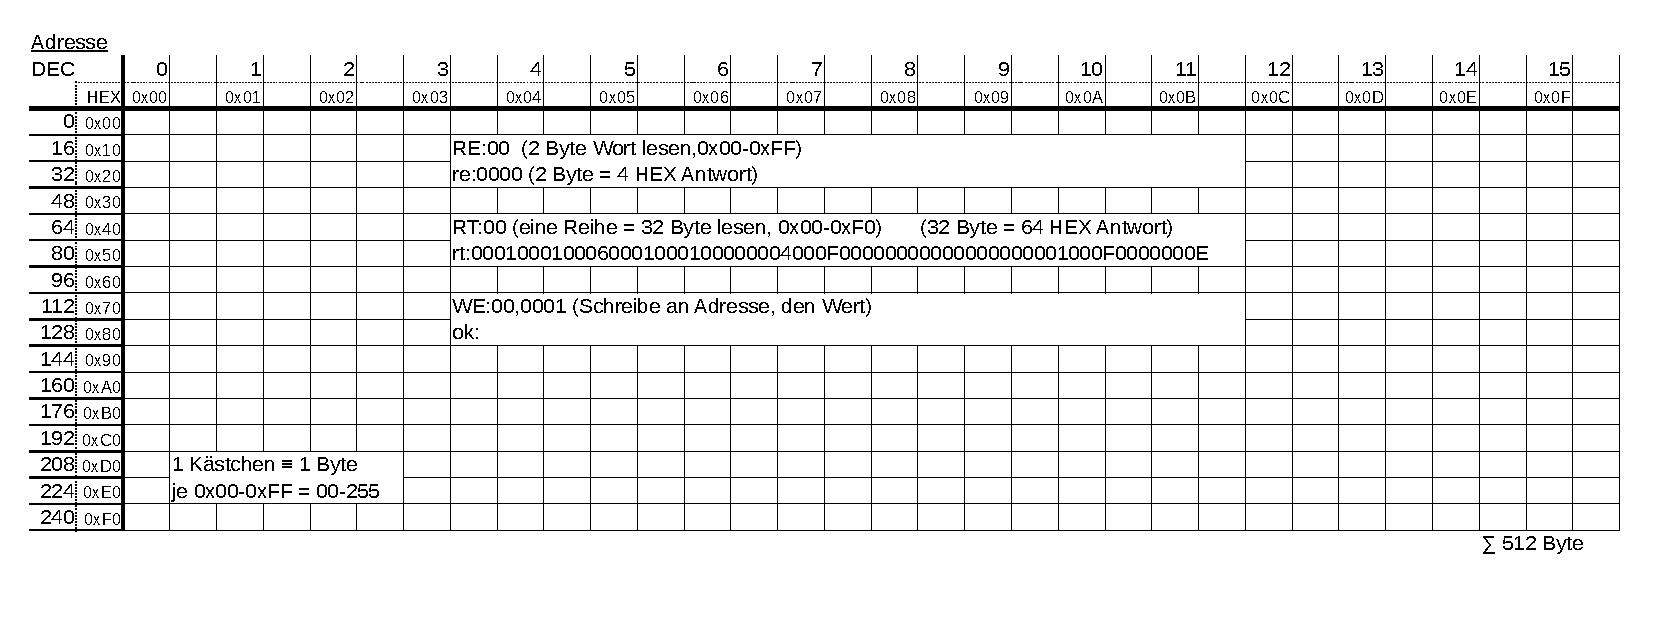
\includegraphics[scale=0.7,trim={0 1.1cm 0 0},clip]{images/chapter_5/Speicher-Schema-Jura-EEPROM}}\\%
    \subfigure[RAM]{\label{subfig:RAM}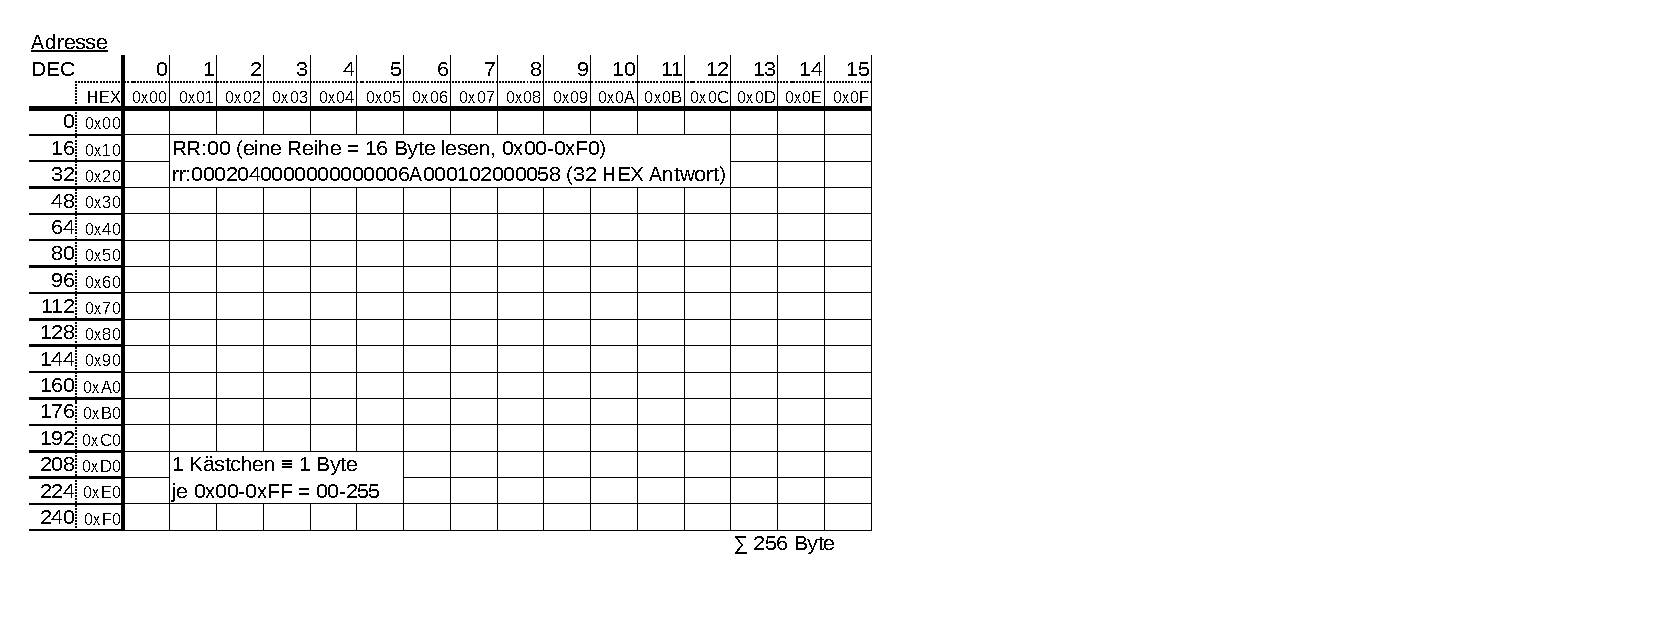
\includegraphics[scale=0.7,trim={0 1.1cm 0 0},clip]{images/chapter_5/Speicher-Schema-Jura-RAM}}%
    \caption{Schematische Darstellung des Speichers vom Kaffeevollautomaten}
    \label{fig:Speicherschema}
\end{sidewaysfigure}

\begin{sidewaystable}
  \footnotesize\centering
  \begin{tabular}[htp]{llllllllll}
  \THc{1}{l}{Funktion} &
  \THc{1}{c}{\rotatebox{50}{Maschine an}} &
  \THc{1}{c}{\rotatebox{50}{Schale fehlt}} &
  \THc{1}{c}{\rotatebox{50}{Schale leeren}} &
  \THc{1}{c}{\rotatebox{50}{Trester leeren}} &
  \THc{1}{c}{\rotatebox{50}{Wasser füllen}} &
  \THc{1}{c}{\rotatebox{50}{Gerät reinigen}} &
  \THc{1}{c}{\rotatebox{50}{Maschine spült}} &
  \THc{1}{c}{\rotatebox{50}{Abschließend spülen}} &
  \THc{1}{c}{\rotatebox{50}{Tassenbeleuchtung}} \\

%
  \TRhc{1}{l}{\textbf{Byte}} &
  \TRhc{1}{l}{\wort{03}} &
  \TRhc{1}{l}{\wort{0E}} &
  \TRhc{1}{l}{\wort{04}} &
  \TRhc{1}{l}{\wort{04}} &
  \TRhc{1}{l}{\wort{04}} &
  \TRhc{1}{l}{\wort{10}} &
  \TRhc{1}{l}{\wort{03}} &
  \TRhc{1}{l}{\wort{0D}} &
  \TRhc{1}{l}{\wort{0F}} \\
  
  Bit &
  \immer{\bitTrue{2}} &
  \immer{\bitTrue{2}} &
  \geteilt{\bitTrue{3}} &
  \bitTrue{5} &
  \geteilt{\bitTrue{3}} &
  \bitTrue{7} &
  \geteilt{\bitTrue{6,3,1}} &
  \bitTrue{3 oder 2} &
  \bitTrue{2 oder 1} \\
  
  \belowbodyrule
%
  \TRhc{1}{l}{\textbf{Byte}} &
  \TRhc{1}{l}{\wort{05}} &
  \TRhc{1}{l}{\wort{16}} &
  \TRhc{1}{l}{\wort{0E}} &
  \TRhc{1}{l}{\wort{0E}} &
  \TRhc{1}{l}{\wort{0E}} &
  \TRhc{1}{l}{\wort{22}} &
  \TRhc{1}{l}{\wort{13}} &
  \TRhc{1}{l}{} &
  \TRhc{1}{l}{} \\
  
  Bit &
  \immer{\bitTrue{5}} &
  \bitFalse{0} &
  \immer{\bitTrue{4}} &
  \bitTrue{5} &
  \immer{\bitTrue{6}} &
  \bitTrue{4} &
  \bitTrue{3,1} &
   &
   \\
  
  \belowbodyrule
%
  \TRhc{1}{l}{\textbf{Byte}} &
  \TRhc{1}{l}{\wort{16}} &
  \TRhc{1}{l}{\wort{29}} &
  \TRhc{1}{l}{\wort{1B}} &
  \TRhc{1}{l}{\wort{80}} &
  \TRhc{1}{l}{\wort{0F}} &
  \TRhc{1}{l}{} &
  \TRhc{1}{l}{\wort{17}} &
  \TRhc{1}{l}{} &
  \TRhc{1}{l}{} \\
  
  Bit &
  \immer{\bitTrue{1}} &
  \immer{\bitFalse{2}} &
  \immer{\bitTrue{1}} &
  \immer{\bitTrue{1,0}} &
  \immer{\bitFalse{4}} &
   &
  \bitTrue{1} &
   &
   \\
  
  \belowbodyrule
%
  \TRhc{1}{l}{\textbf{Byte}} &
  \TRhc{1}{l}{\wort{44}} &
  \TRhc{1}{l}{\wort{69}} &
  \TRhc{1}{l}{\wort{29}} &
  \TRhc{1}{l}{} &
  \TRhc{1}{l}{\wort{4C}} &
  \TRhc{1}{l}{} &
  \TRhc{1}{l}{\wort{62}} &
  \TRhc{1}{l}{} &
  \TRhc{1}{l}{} \\
  
  Bit &
  \immer{\bitTrue{0}} &
  \bitFalse{0} &
  \immer{\bitTrue{6-3}} &
   &
  \geteilt{\bitFalse{0}} &
   &
  \geteilt{\bitTrue{1}} &
   &
   \\
  
  \belowbodyrule
%
  \TRhc{1}{l}{\textbf{Byte}} &
  \TRhc{1}{l}{} &
  \TRhc{1}{l}{} &
  \TRhc{1}{l}{\wort{2B}} &
  \TRhc{1}{l}{} &
  \TRhc{1}{l}{\wort{91}} &
  \TRhc{1}{l}{} &
  \TRhc{1}{l}{} &
  \TRhc{1}{l}{} &
  \TRhc{1}{l}{} \\
  
  Bit &
   &
   &
  \immer{\bitTrue{6-3}} &
   &
  \geteilt{\bitFalse{1}} &
   &
   &
   &
   \\
  
  \belowbodyrule
%
  \TRhc{1}{l}{\textbf{Byte}} &
  \TRhc{1}{l}{\wort{1A}} &
  \TRhc{1}{l}{} &
  \TRhc{1}{l}{} &
  \TRhc{1}{l}{} &
  \TRhc{1}{l}{} &
  \TRhc{1}{l}{} &
  \TRhc{1}{l}{\wort{68}} &
  \TRhc{1}{l}{} &
  \TRhc{1}{l}{} \\
  
  Bit &
  \immer{\bitFalse{2}} &
   &
   &
   &
   &
   &
  \geteilt{\bitTrue{6}} &
   &
   \\
  
  Bit &
  \immer{\bitTrue{1,0}} &
   &
   &
   &
   &
   &
  \geteilt{\bitFalse{5,4}} &
   &
   \\
  \belowbodyrule
  \end{tabular}
  \caption{Speicherpositionen im RAM (1)}
  \label{tbl:RAM1}
\end{sidewaystable}
\begin{sidewaystable}
  \footnotesize\centering
  \begin{tabular}[htp]{lllllllllll}
  \THc{1}{l}{Funktion} &
  \THc{1}{c}{\rotatebox{50}{Filter wechseln}} &
  \THc{1}{c}{\rotatebox{50}{Hahn offen}} &
  \THc{1}{c}{\rotatebox{50}{Teeportion}} &
  \THc{1}{c}{\rotatebox{50}{Dampfbezug}} &
  \THc{1}{c}{\rotatebox{50}{Wasserdampfportion}} &
  \THc{1}{c}{\rotatebox{50}{Pulver füllen}} &
  \THc{1}{c}{\rotatebox{50}{Bohnen füllen}} &
  \THc{3}{c}{\rotatebox{50}{Zubereitung}} \\
  
  \THsub{1}{l}{} &
  \THsub{1}{l}{} &
  \THsub{1}{l}{} &
  \THsub{1}{l}{} &
  \THsub{1}{l}{} &
  \THsub{1}{l}{} &
  \THsub{1}{l}{} &
  \THsub{1}{l}{} &
  \THsub{1}{c}{immer} &
  \THsub{1}{c}{1. Schritt} &
  \THsub{1}{c}{2. Schritt} \\

%
  \TRhc{1}{l}{\textbf{Byte}} &
  \TRhc{1}{l}{\wort{10}} &
  \TRhc{1}{l}{\wort{04}} &
  \TRhc{1}{l}{\wort{03}} &
  \TRhc{1}{l}{\wort{04}} &
  \TRhc{1}{l}{\wort{03}} &
  \TRhc{1}{l}{\wort{04}} &
  \TRhc{1}{l}{\wort{0E}} &
  \TRhc{1}{l}{} &
  \TRhc{1}{l}{} &
  \TRhc{1}{l}{\wort{03}} \\
  
  Bit &
  \bitTrue{5} &
  \geteilt{\bitTrue{3}} &
  \geteilt{\bitTrue{6}} &
  \geteilt{\bitTrue{3}} &
  \geteilt{\bitTrue{3}} &
  \bitTrue{0} &
  \bitTrue{7} &
   &
   &
  \bitTrue{1} \\
  
  \belowbodyrule
%
  \TRhc{1}{l}{\textbf{Byte}} &
  \TRhc{1}{l}{\wort{22}} &
  \TRhc{1}{l}{\wort{0F}} &
  \TRhc{1}{l}{\wort{0B}} &
  \TRhc{1}{l}{\wort{0B}} &
  \TRhc{1}{l}{\wort{0B}} &
  \TRhc{1}{l}{} &
  \TRhc{1}{l}{} &
  \TRhc{1}{l}{} &
  \TRhc{1}{l}{} &
  \TRhc{1}{l}{\wort{0B}} \\
  
  Bit &
  \bitTrue{3} &
  \immer{\bitFalse{6}} &
  \geteilt{\bitFalse{3}} &
  \geteilt{\bitFalse{3}} &
  \geteilt{\bitFalse{3}} &
   &
   &
   &
   &
  \geteilt{\bitFalse{3}} \\
    
  \belowbodyrule
%
  \TRhc{1}{l}{\textbf{Byte}} &
  \TRhc{1}{l}{\wort{F8}} &
  \TRhc{1}{l}{\wort{4C}} &
  \TRhc{1}{l}{\wort{0F}} &
  \TRhc{1}{l}{\wort{13}} &
  \TRhc{1}{l}{\wort{13}} &
  \TRhc{1}{l}{} &
  \TRhc{1}{l}{} &
  \TRhc{1}{l}{} &
  \TRhc{1}{l}{} &
  \TRhc{1}{l}{\wort{17}} \\
  
  Bit &
  \immer{\bitTrue{0}} &
  \geteilt{\bitFalse{0}} &
  \immer{\bitTrue{5}} &
  \bitTrue{2-0} &
  \bitTrue{2,0} &
   &
   &
   &
   &
  \bitTrue{3} \\
  
  \belowbodyrule
%
  \TRhc{1}{l}{\textbf{Byte}} &
  \TRhc{1}{l}{} &
  \TRhc{1}{l}{\wort{4D}} &
  \TRhc{1}{l}{\wort{4C}} &
  \TRhc{1}{l}{\wort{49}} &
  \TRhc{1}{l}{\wort{49}} &
  \TRhc{1}{l}{} &
  \TRhc{1}{l}{} &
  \TRhc{1}{l}{} &
  \TRhc{1}{l}{} &
  \TRhc{1}{l}{\wort{62}} \\
  
  Bit &
   &
  \bitTrue{3,1} &
  \geteilt{\bitFalse{0}} &
  \geteilt{\bitTrue{0}} &
  \geteilt{\bitTrue{0}} &
   &
   &
   &
   &
  \geteilt{\bitTrue{1}} \\
  
  \belowbodyrule
%
  \TRhc{1}{l}{\textbf{Byte}} &
  \TRhc{1}{l}{} &
  \TRhc{1}{l}{} &
  \TRhc{1}{l}{\wort{68}} &
  \TRhc{1}{l}{\wort{4C}} &
  \TRhc{1}{l}{\wort{4C}} &
  \TRhc{1}{l}{} &
  \TRhc{1}{l}{} &
  \TRhc{1}{l}{} &
  \TRhc{1}{l}{} &
  \TRhc{1}{l}{\wort{68}} \\
  
  Bit &
   &
   &
  \geteilt{\bitTrue{6}} &
  \geteilt{\bitFalse{0}} &
  \geteilt{\bitFalse{0}} &
   &
   &
   &
   &
  \geteilt{\bitFalse{5}} \\
  
  \belowbodyrule
%
  \TRhc{1}{l}{\textbf{Byte}} &
  \TRhc{1}{l}{\wort{F9}} &
  \TRhc{1}{l}{} &
  \TRhc{1}{l}{\wort{4D}} &
  \TRhc{1}{l}{} &
  \TRhc{1}{l}{} &
  \TRhc{1}{l}{} &
  \TRhc{1}{l}{} &
  \TRhc{1}{l}{\wort{0A}} &
  \TRhc{1}{l}{\wort{03}} &
  \TRhc{1}{l}{} \\
  
  Bit &
  \bitTrue{7,6,5,4,2} &
   &
  \bitFalse{3,1} &
   &
   &
   &
   &
  \bitTrue{6} &
  \bitTrue{7,4} &
   \\
  
   &
  (\wert{$0_{10} \rightarrow 244_{10}$}) &
   &
  \bitTrue{0} &
   &
   &
   &
   &
  (2-0: "`Kaffee"') &
  (7 nicht manuell) &
   \\
  \belowbodyrule
  \end{tabular}
  \caption{Speicherpositionen im RAM (2)}
  \label{tbl:RAM2}
\end{sidewaystable}

\begin{sidewaysfigure}
  \begin{center}
    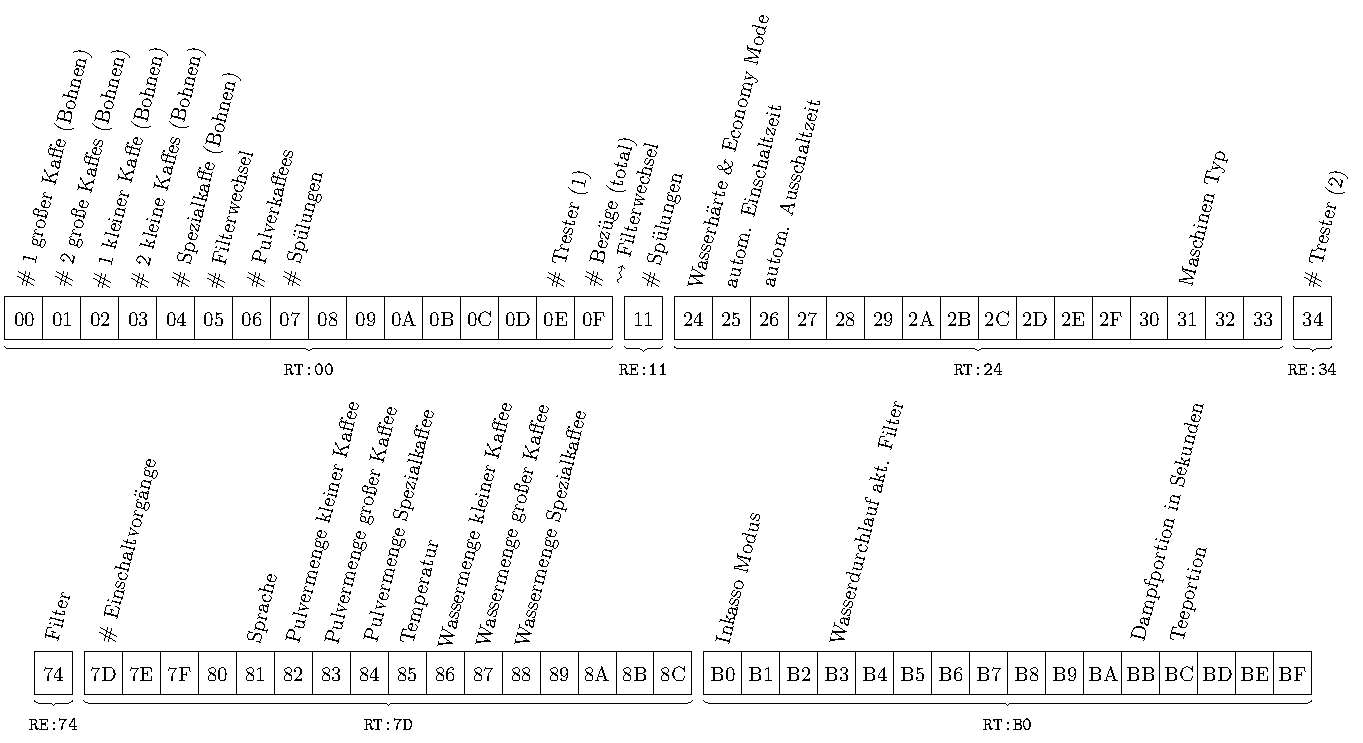
\includegraphics[scale=0.94]{images/chapter_5/API-EEPROM}
    \caption{Abgefragte Speicherstellen für die API im EEPROM (1 Kästchen $\equiv$ 1 Wort)}
    \label{fig:API-EEPROM}
  \end{center}
\end{sidewaysfigure}
\begin{sidewaysfigure}
  \begin{center}
    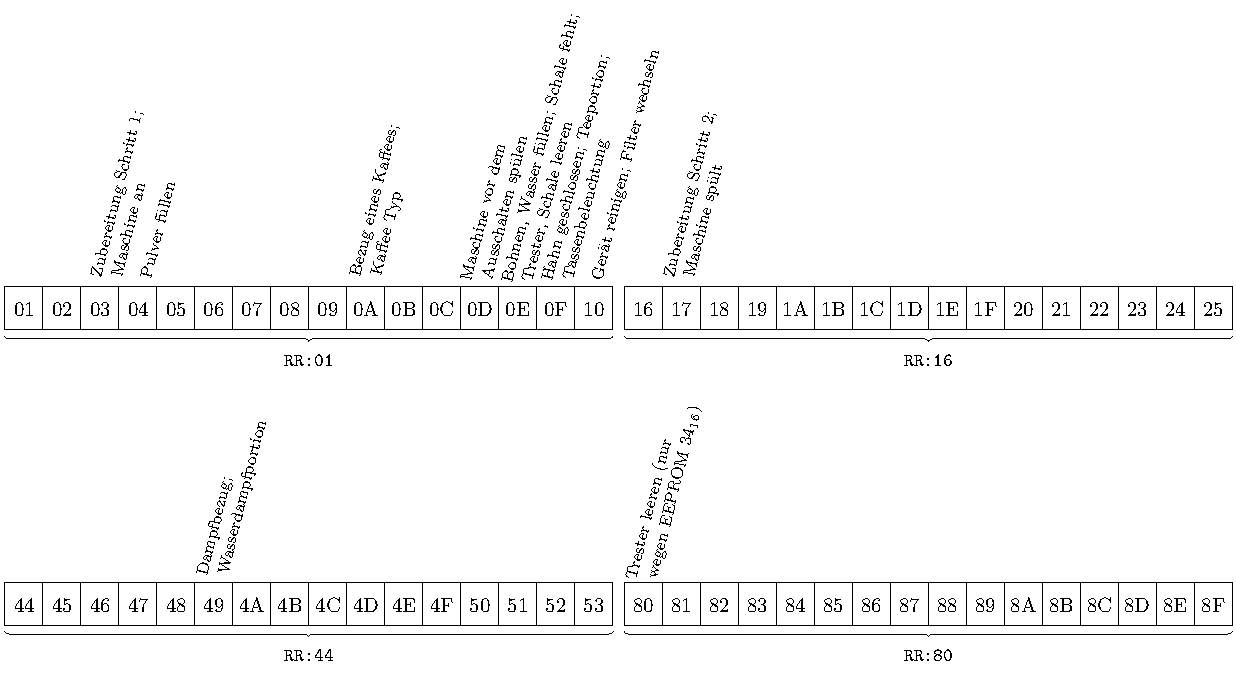
\includegraphics[scale=1]{images/chapter_5/API-RAM}
    \caption{Abgefragte Speicherstellen für die API im RAM (1 Kästchen $\equiv$ 1 Byte)}
    \label{fig:API-RAM}
  \end{center}
\end{sidewaysfigure}

\begin{tuhhtable}
  \newcommand{\display}[1]{\includegraphics[height=2ex]{images/chapter_5/display/#1.png}}
  \footnotesize\centering
  \begin{tabular}[tp]{rrcc   L{1mm}   rrcc}
%
  \THc{3}{c}{ASCII} & \THc{1}{c}{Kaffeevollautomat} &   \TRhc{1}{l}{}   &   \THc{3}{c}{ASCII} & \THc{1}{c}{Kaffeevollautomat} \\
  \THsub{1}{r}{hex} & \THsub{1}{r}{dez} & \THsub{1}{c}{Zeichen} & \THsub{1}{c}{Display} &   \TRhc{1}{l}{}   & \THsub{1}{r}{hex} & \THsub{1}{r}{dez} & \THsub{1}{c}{Zeichen} & \THsub{1}{c}{Display} \\
%
%  \abovebodyrule
%
       & {\tiny 0 – 31} & {\tiny$\ldots$} & {\tiny$\ldots$}   & \TRhc{1}{l}{} &   0x41 & 65            & A                          & A \\\TRc
  0x20 & 32             & Leerzeichen     & Leerzeichen       & \TRhc{1}{l}{} &   0x42 & 66            & B                          & B \\
  0x21 & 33             & !               & \_                & \TRhc{1}{l}{} &   0x43 & 67            & C                          & C \\\TRc
  0x22 & 34             & "               & \display{34}      & \TRhc{1}{l}{} &   0x44 & 68            & D                          & D \\
  0x23 & 35             & \#              & \display{35}      & \TRhc{1}{l}{} &   0x45 & 69            & E                          & E \\\TRc
  0x24 & 36             & \$              & \display{36}      & \TRhc{1}{l}{} &   0x46 & 70            & F                          & F \\
  0x25 & 37             & \%              & \display{37}      & \TRhc{1}{l}{} &   0x47 & 71            & G                          & G \\\TRc
  0x26 & 38             & \&              & \display{38}      & \TRhc{1}{l}{} &   0x48 & 72            & H                          & H \\
  0x27 & 39             & '               & \display{39}      & \TRhc{1}{l}{} &   0x49 & 73            & I                          & I \\\TRc
  0x28 & 40             & (               & \display{40}      & \TRhc{1}{l}{} &   0x4A & 74            & J                          & J \\
  0x29 & 41             & )               & \display{41}      & \TRhc{1}{l}{} &   0x4B & 75            & K                          & K \\\TRc
  0x2A & 42       & \textasteriskcentered & \display{42}      & \TRhc{1}{l}{} &   0x4C & 76            & L                          & L \\
  0x2B & 43             & +               & +                 & \TRhc{1}{l}{} &   0x4D & 77            & M                          & M \\\TRc
  0x2C & 44             & ,               & ,                 & \TRhc{1}{l}{} &   0x4E & 78            & N                          & N \\
  0x2D & 45             & -               & -                 & \TRhc{1}{l}{} &   0x4F & 79            & O                          & O \\\TRc
  0x2E & 46             & .               & .                 & \TRhc{1}{l}{} &   0x50 & 80            & P                          & P \\
  0x2F & 47             & /               & /                 & \TRhc{1}{l}{} &   0x51 & 81            & Q                          & Q \\\TRc
  0x30 & 48             & 0               & 0                 & \TRhc{1}{l}{} &   0x52 & 82            & R                          & R \\
  0x31 & 49             & 1               & 1                 & \TRhc{1}{l}{} &   0x53 & 83            & S                          & S \\\TRc
  0x32 & 50             & 2               & 2                 & \TRhc{1}{l}{} &   0x54 & 84            & T                          & T \\
  0x33 & 51             & 3               & 3                 & \TRhc{1}{l}{} &   0x55 & 85            & U                          & U \\\TRc
  0x34 & 52             & 4               & 4                 & \TRhc{1}{l}{} &   0x56 & 86            & V                          & V \\
  0x35 & 53             & 5               & 5                 & \TRhc{1}{l}{} &   0x57 & 87            & W                          & W \\\TRc
  0x36 & 54             & 6               & 6                 & \TRhc{1}{l}{} &   0x58 & 88            & X                          & X \\
  0x37 & 55             & 7               & 7                 & \TRhc{1}{l}{} &   0x59 & 89            & Y                          & Y \\\TRc
  0x38 & 56             & 8               & 8                 & \TRhc{1}{l}{} &   0x5A & 90            & Z                          & Z \\
  0x39 & 57             & 9               & 9                 & \TRhc{1}{l}{} &   0x5B & 91            & [                          & \display{91} \\\TRc
  0x3A & 58             & :               & :                 & \TRhc{1}{l}{} &   0x5C & 92            & \textbackslash             & \display{92} \\
  0x3B & 59             & ;               & ;                 & \TRhc{1}{l}{} &   0x5D & 93            & ]                          & \display{93} \\\TRc
  0x3C & 60             & <               & <                 & \TRhc{1}{l}{} &   0x5E & 94            & \^{}                       & \display{94} \\
  0x3D & 61             & =               & =                 & \TRhc{1}{l}{} &   0x5F & 95            & \_                         & \display{95} \\\TRc
  0x3E & 62             & >               & >                 & \TRhc{1}{l}{} &   0x60 & 96            & `                          & \display{96} \\
  0x3F & 63             & ?               & ?                 & \TRhc{1}{l}{} &        & {\tiny97-127} & {\tiny a-z \{ | \} $\sim$} & {\tiny$\ldots$} \\\TRc
  0x40 & 64             & @               & \display{64}      & \TRhc{1}{l}{} &        &               &                            &   \\
%
   \belowbodyrule
%
  \end{tabular}
  \caption{Verfügbarer Zeichensatz des Displays}
  \label{tbl:Displaysymbole}
\end{tuhhtable}

  \chapter{Inhalt der CD}

\begin{tuhhtable}
  \footnotesize\centering
  \begin{tabular}[tb]{L{.35\textwidth}L{.55\textwidth}}
    \THc{1}{c}{Inhalt}                    & \THc{1}{c}{Beschreibung} \\
    \abovebodyrule
    thesis.pdf                            & Diese Arbeit in digitaler Form \\\TRc
    JuraCoffeeMemory/                     & Das entwickelte Projekt \\
    JuraCoffeeMemory/arduino/arduino.ino  & Das Arduino Skript aus \cite{GitCoffeeMachine} \\\TRc
    JuraCoffeeMemory/data/                & Die aufgenommenen Speicherauszüge im JSON Format \\
    JuraCoffeeMemory/doxygen/             & Die Doxygen Dokumentation \\\TRc
    JuraCoffeeMemory/manual\_jura/        & Handbuch und Abbildung des Kaffeevollautomaten aus \cite{GitCoffeeMachine} \\
    JuraCoffeeMemory/result/              & Ergebnisse der Auswertung \\\TRc
    JuraCoffeeMemory/tools/               & Kleine Helfer-Programme und Codeschnipsel \\
    JuraCoffeeMemory/website/             & Die Webseite zur Visualisierung \\\TRc
    \belowbodyrule
  \end{tabular}
  \caption{Inhalt der CD}
  \label{tbl:elements}
\end{tuhhtable}

\end{tuhhappendix}


% The End
\end{document}
